% Options for packages loaded elsewhere
\PassOptionsToPackage{unicode}{hyperref}
\PassOptionsToPackage{hyphens}{url}
%
\documentclass[
]{article}
\usepackage{amsmath,amssymb}
\usepackage{lmodern}
\usepackage{iftex}
\ifPDFTeX
  \usepackage[T1]{fontenc}
  \usepackage[utf8]{inputenc}
  \usepackage{textcomp} % provide euro and other symbols
\else % if luatex or xetex
  \usepackage{unicode-math}
  \defaultfontfeatures{Scale=MatchLowercase}
  \defaultfontfeatures[\rmfamily]{Ligatures=TeX,Scale=1}
\fi
% Use upquote if available, for straight quotes in verbatim environments
\IfFileExists{upquote.sty}{\usepackage{upquote}}{}
\IfFileExists{microtype.sty}{% use microtype if available
  \usepackage[]{microtype}
  \UseMicrotypeSet[protrusion]{basicmath} % disable protrusion for tt fonts
}{}
\makeatletter
\@ifundefined{KOMAClassName}{% if non-KOMA class
  \IfFileExists{parskip.sty}{%
    \usepackage{parskip}
  }{% else
    \setlength{\parindent}{0pt}
    \setlength{\parskip}{6pt plus 2pt minus 1pt}}
}{% if KOMA class
  \KOMAoptions{parskip=half}}
\makeatother
\usepackage{xcolor}
\usepackage[margin=1in]{geometry}
\usepackage{color}
\usepackage{fancyvrb}
\newcommand{\VerbBar}{|}
\newcommand{\VERB}{\Verb[commandchars=\\\{\}]}
\DefineVerbatimEnvironment{Highlighting}{Verbatim}{commandchars=\\\{\}}
% Add ',fontsize=\small' for more characters per line
\usepackage{framed}
\definecolor{shadecolor}{RGB}{248,248,248}
\newenvironment{Shaded}{\begin{snugshade}}{\end{snugshade}}
\newcommand{\AlertTok}[1]{\textcolor[rgb]{0.94,0.16,0.16}{#1}}
\newcommand{\AnnotationTok}[1]{\textcolor[rgb]{0.56,0.35,0.01}{\textbf{\textit{#1}}}}
\newcommand{\AttributeTok}[1]{\textcolor[rgb]{0.77,0.63,0.00}{#1}}
\newcommand{\BaseNTok}[1]{\textcolor[rgb]{0.00,0.00,0.81}{#1}}
\newcommand{\BuiltInTok}[1]{#1}
\newcommand{\CharTok}[1]{\textcolor[rgb]{0.31,0.60,0.02}{#1}}
\newcommand{\CommentTok}[1]{\textcolor[rgb]{0.56,0.35,0.01}{\textit{#1}}}
\newcommand{\CommentVarTok}[1]{\textcolor[rgb]{0.56,0.35,0.01}{\textbf{\textit{#1}}}}
\newcommand{\ConstantTok}[1]{\textcolor[rgb]{0.00,0.00,0.00}{#1}}
\newcommand{\ControlFlowTok}[1]{\textcolor[rgb]{0.13,0.29,0.53}{\textbf{#1}}}
\newcommand{\DataTypeTok}[1]{\textcolor[rgb]{0.13,0.29,0.53}{#1}}
\newcommand{\DecValTok}[1]{\textcolor[rgb]{0.00,0.00,0.81}{#1}}
\newcommand{\DocumentationTok}[1]{\textcolor[rgb]{0.56,0.35,0.01}{\textbf{\textit{#1}}}}
\newcommand{\ErrorTok}[1]{\textcolor[rgb]{0.64,0.00,0.00}{\textbf{#1}}}
\newcommand{\ExtensionTok}[1]{#1}
\newcommand{\FloatTok}[1]{\textcolor[rgb]{0.00,0.00,0.81}{#1}}
\newcommand{\FunctionTok}[1]{\textcolor[rgb]{0.00,0.00,0.00}{#1}}
\newcommand{\ImportTok}[1]{#1}
\newcommand{\InformationTok}[1]{\textcolor[rgb]{0.56,0.35,0.01}{\textbf{\textit{#1}}}}
\newcommand{\KeywordTok}[1]{\textcolor[rgb]{0.13,0.29,0.53}{\textbf{#1}}}
\newcommand{\NormalTok}[1]{#1}
\newcommand{\OperatorTok}[1]{\textcolor[rgb]{0.81,0.36,0.00}{\textbf{#1}}}
\newcommand{\OtherTok}[1]{\textcolor[rgb]{0.56,0.35,0.01}{#1}}
\newcommand{\PreprocessorTok}[1]{\textcolor[rgb]{0.56,0.35,0.01}{\textit{#1}}}
\newcommand{\RegionMarkerTok}[1]{#1}
\newcommand{\SpecialCharTok}[1]{\textcolor[rgb]{0.00,0.00,0.00}{#1}}
\newcommand{\SpecialStringTok}[1]{\textcolor[rgb]{0.31,0.60,0.02}{#1}}
\newcommand{\StringTok}[1]{\textcolor[rgb]{0.31,0.60,0.02}{#1}}
\newcommand{\VariableTok}[1]{\textcolor[rgb]{0.00,0.00,0.00}{#1}}
\newcommand{\VerbatimStringTok}[1]{\textcolor[rgb]{0.31,0.60,0.02}{#1}}
\newcommand{\WarningTok}[1]{\textcolor[rgb]{0.56,0.35,0.01}{\textbf{\textit{#1}}}}
\usepackage{graphicx}
\makeatletter
\def\maxwidth{\ifdim\Gin@nat@width>\linewidth\linewidth\else\Gin@nat@width\fi}
\def\maxheight{\ifdim\Gin@nat@height>\textheight\textheight\else\Gin@nat@height\fi}
\makeatother
% Scale images if necessary, so that they will not overflow the page
% margins by default, and it is still possible to overwrite the defaults
% using explicit options in \includegraphics[width, height, ...]{}
\setkeys{Gin}{width=\maxwidth,height=\maxheight,keepaspectratio}
% Set default figure placement to htbp
\makeatletter
\def\fps@figure{htbp}
\makeatother
\setlength{\emergencystretch}{3em} % prevent overfull lines
\providecommand{\tightlist}{%
  \setlength{\itemsep}{0pt}\setlength{\parskip}{0pt}}
\setcounter{secnumdepth}{-\maxdimen} % remove section numbering
\ifLuaTeX
  \usepackage{selnolig}  % disable illegal ligatures
\fi
\IfFileExists{bookmark.sty}{\usepackage{bookmark}}{\usepackage{hyperref}}
\IfFileExists{xurl.sty}{\usepackage{xurl}}{} % add URL line breaks if available
\urlstyle{same} % disable monospaced font for URLs
\hypersetup{
  pdftitle={final project},
  pdfauthor={Takuto Yoshida},
  hidelinks,
  pdfcreator={LaTeX via pandoc}}

\title{final project}
\author{Takuto Yoshida}
\date{2022-12-13}

\begin{document}
\maketitle

\#\textbf{Final project} \#\# \textbf{Introduction} Titanic was the name
of a British luxury liner with a gross tonnage of 46,328 tons. On her
maiden voyage to New York in 1912, she collided with an iceberg off the
coast of Newfoundland on April 14 and sank. It was the world's largest
maritime accident, claiming the lives of 1514 of the 22008 people on
board. This was the first time that the internationally established
distress signal ``SOS'' was sent out. Later, this maritime accident was
featured in Hollywood, where Leonardo DiCaprio and Kate Winslet gave
glamorous and tragic performances. The film won 11 Academy Awards in
1998, including Best Picture, and its total U.S. box office gross of
\$659,363,944 ranks seventh on the U.S. all-time list. Predicting the
Titanic's survivors is the gateway problem for Kaggle, the world's
largest platform for data scientists. Using this data set, I created
multiple models and evaluated their performance to determine which model
performed the best.

\hypertarget{objective}{%
\subsubsection{\texorpdfstring{\textbf{Objective}}{Objective}}\label{objective}}

What I have done in this project is the following. * To make the data
set tidy so that it can be analyzed. * Evaluate each variable and create
variables to be used for forecasting. * Create multiple models and
select the model with the best predictive performance.

\hypertarget{methods}{%
\subsubsection{\texorpdfstring{\textbf{Methods}}{Methods}}\label{methods}}

For each variable, I evaluated its association with mortality to
determine if it was useful for prediction. I created variables that I
considered useful for forecasting. If there were missing values, I
substituted values in multiple ways to ensure that there were no missing
values in the data. Finally, multiple machine learning models were
created using these variables, and their predictive ability was
evaluated.

\hypertarget{results}{%
\subsection{\texorpdfstring{\textbf{Results}}{Results}}\label{results}}

\hypertarget{importing-combining-data-overview}{%
\subsubsection{\texorpdfstring{\textbf{Importing, Combining, Data
Overview}}{Importing, Combining, Data Overview}}\label{importing-combining-data-overview}}

\begin{Shaded}
\begin{Highlighting}[]
\CommentTok{\# Install packages}
\CommentTok{\# install.packages("kernlab")}
\CommentTok{\# install.packages("C50")}
\CommentTok{\# install.packages("tictoc")}

\CommentTok{\# Make the following libraries available}
\FunctionTok{library}\NormalTok{(}\StringTok{\textquotesingle{}readr\textquotesingle{}}\NormalTok{) }
\FunctionTok{library}\NormalTok{(}\StringTok{\textquotesingle{}dplyr\textquotesingle{}}\NormalTok{) }
\end{Highlighting}
\end{Shaded}

\begin{verbatim}
## 
## Attaching package: 'dplyr'
\end{verbatim}

\begin{verbatim}
## The following objects are masked from 'package:stats':
## 
##     filter, lag
\end{verbatim}

\begin{verbatim}
## The following objects are masked from 'package:base':
## 
##     intersect, setdiff, setequal, union
\end{verbatim}

\begin{Shaded}
\begin{Highlighting}[]
\FunctionTok{library}\NormalTok{(}\StringTok{\textquotesingle{}ggplot2\textquotesingle{}}\NormalTok{) }
\FunctionTok{library}\NormalTok{(}\StringTok{\textquotesingle{}gridExtra\textquotesingle{}}\NormalTok{)}
\end{Highlighting}
\end{Shaded}

\begin{verbatim}
## 
## Attaching package: 'gridExtra'
\end{verbatim}

\begin{verbatim}
## The following object is masked from 'package:dplyr':
## 
##     combine
\end{verbatim}

\begin{Shaded}
\begin{Highlighting}[]
\FunctionTok{library}\NormalTok{(}\StringTok{\textquotesingle{}tictoc\textquotesingle{}}\NormalTok{) }
\FunctionTok{library}\NormalTok{(}\StringTok{\textquotesingle{}caret\textquotesingle{}}\NormalTok{) }
\end{Highlighting}
\end{Shaded}

\begin{verbatim}
## Loading required package: lattice
\end{verbatim}

\begin{Shaded}
\begin{Highlighting}[]
\FunctionTok{library}\NormalTok{(}\StringTok{\textquotesingle{}mice\textquotesingle{}}\NormalTok{)}
\end{Highlighting}
\end{Shaded}

\begin{verbatim}
## 
## Attaching package: 'mice'
\end{verbatim}

\begin{verbatim}
## The following object is masked from 'package:stats':
## 
##     filter
\end{verbatim}

\begin{verbatim}
## The following objects are masked from 'package:base':
## 
##     cbind, rbind
\end{verbatim}

\begin{Shaded}
\begin{Highlighting}[]
\FunctionTok{library}\NormalTok{(}\StringTok{\textquotesingle{}randomForest\textquotesingle{}}\NormalTok{)}
\end{Highlighting}
\end{Shaded}

\begin{verbatim}
## randomForest 4.7-1.1
\end{verbatim}

\begin{verbatim}
## Type rfNews() to see new features/changes/bug fixes.
\end{verbatim}

\begin{verbatim}
## 
## Attaching package: 'randomForest'
\end{verbatim}

\begin{verbatim}
## The following object is masked from 'package:gridExtra':
## 
##     combine
\end{verbatim}

\begin{verbatim}
## The following object is masked from 'package:ggplot2':
## 
##     margin
\end{verbatim}

\begin{verbatim}
## The following object is masked from 'package:dplyr':
## 
##     combine
\end{verbatim}

\begin{Shaded}
\begin{Highlighting}[]
\FunctionTok{library}\NormalTok{(}\StringTok{\textquotesingle{}glmnet\textquotesingle{}}\NormalTok{)}
\end{Highlighting}
\end{Shaded}

\begin{verbatim}
## Loading required package: Matrix
\end{verbatim}

\begin{verbatim}
## Loaded glmnet 4.1-4
\end{verbatim}

\begin{Shaded}
\begin{Highlighting}[]
\FunctionTok{library}\NormalTok{(}\StringTok{\textquotesingle{}kernlab\textquotesingle{}}\NormalTok{)}
\end{Highlighting}
\end{Shaded}

\begin{verbatim}
## 
## Attaching package: 'kernlab'
\end{verbatim}

\begin{verbatim}
## The following object is masked from 'package:mice':
## 
##     convergence
\end{verbatim}

\begin{verbatim}
## The following object is masked from 'package:tictoc':
## 
##     size
\end{verbatim}

\begin{verbatim}
## The following object is masked from 'package:ggplot2':
## 
##     alpha
\end{verbatim}

\begin{Shaded}
\begin{Highlighting}[]
\FunctionTok{library}\NormalTok{(}\StringTok{\textquotesingle{}C50\textquotesingle{}}\NormalTok{)}
\FunctionTok{library}\NormalTok{(}\StringTok{\textquotesingle{}pROC\textquotesingle{}}\NormalTok{)}
\end{Highlighting}
\end{Shaded}

\begin{verbatim}
## Type 'citation("pROC")' for a citation.
\end{verbatim}

\begin{verbatim}
## 
## Attaching package: 'pROC'
\end{verbatim}

\begin{verbatim}
## The following objects are masked from 'package:stats':
## 
##     cov, smooth, var
\end{verbatim}

\begin{Shaded}
\begin{Highlighting}[]
\FunctionTok{library}\NormalTok{(}\StringTok{\textquotesingle{}Matrix\textquotesingle{}}\NormalTok{)}
\FunctionTok{library}\NormalTok{(}\StringTok{\textquotesingle{}tidyverse\textquotesingle{}}\NormalTok{)}
\end{Highlighting}
\end{Shaded}

\begin{verbatim}
## -- Attaching packages --------------------------------------- tidyverse 1.3.2 --
\end{verbatim}

\begin{verbatim}
## v tibble  3.1.8     v stringr 1.4.1
## v tidyr   1.2.1     v forcats 0.5.2
## v purrr   0.3.5     
## -- Conflicts ------------------------------------------ tidyverse_conflicts() --
## x kernlab::alpha()        masks ggplot2::alpha()
## x randomForest::combine() masks gridExtra::combine(), dplyr::combine()
## x purrr::cross()          masks kernlab::cross()
## x tidyr::expand()         masks Matrix::expand()
## x mice::filter()          masks dplyr::filter(), stats::filter()
## x dplyr::lag()            masks stats::lag()
## x purrr::lift()           masks caret::lift()
## x randomForest::margin()  masks ggplot2::margin()
## x tidyr::pack()           masks Matrix::pack()
## x tidyr::unpack()         masks Matrix::unpack()
\end{verbatim}

\begin{Shaded}
\begin{Highlighting}[]
\FunctionTok{library}\NormalTok{(}\StringTok{\textquotesingle{}stringr\textquotesingle{}}\NormalTok{)}
\FunctionTok{library}\NormalTok{(}\StringTok{\textquotesingle{}ranger\textquotesingle{}}\NormalTok{)}
\end{Highlighting}
\end{Shaded}

\begin{verbatim}
## 
## Attaching package: 'ranger'
## 
## The following object is masked from 'package:randomForest':
## 
##     importance
\end{verbatim}

\begin{Shaded}
\begin{Highlighting}[]
\FunctionTok{library}\NormalTok{(}\StringTok{\textquotesingle{}e1071\textquotesingle{}}\NormalTok{)}
\FunctionTok{library}\NormalTok{(}\StringTok{\textquotesingle{}corrplot\textquotesingle{}}\NormalTok{)}
\end{Highlighting}
\end{Shaded}

\begin{verbatim}
## corrplot 0.92 loaded
\end{verbatim}

\begin{Shaded}
\begin{Highlighting}[]
\FunctionTok{library}\NormalTok{(}\StringTok{\textquotesingle{}scales\textquotesingle{}}\NormalTok{)}
\end{Highlighting}
\end{Shaded}

\begin{verbatim}
## 
## Attaching package: 'scales'
## 
## The following object is masked from 'package:purrr':
## 
##     discard
## 
## The following object is masked from 'package:kernlab':
## 
##     alpha
## 
## The following object is masked from 'package:readr':
## 
##     col_factor
\end{verbatim}

\begin{Shaded}
\begin{Highlighting}[]
\FunctionTok{library}\NormalTok{(}\StringTok{\textquotesingle{}ggthemes\textquotesingle{}}\NormalTok{)}
\end{Highlighting}
\end{Shaded}

\begin{Shaded}
\begin{Highlighting}[]
\CommentTok{\# Importing the dataset}
\FunctionTok{theme\_set}\NormalTok{(}\FunctionTok{theme\_light}\NormalTok{())}
\FunctionTok{setwd}\NormalTok{(}\StringTok{"/Users/yoshidatakuto/Dropbox/HSPH/MPH{-}CLE/BST260/titanic (1)"}\NormalTok{)}
\NormalTok{train\_titanic }\OtherTok{\textless{}{-}} \FunctionTok{read.csv}\NormalTok{(}\StringTok{"test.csv"}\NormalTok{, }\AttributeTok{stringsAsFactors =}\NormalTok{ F) }\SpecialCharTok{\%\textgreater{}\%} \FunctionTok{mutate}\NormalTok{(}\AttributeTok{Test\_Data =} \DecValTok{0}\NormalTok{)}
\NormalTok{test\_titanic }\OtherTok{\textless{}{-}} \FunctionTok{read.csv}\NormalTok{(}\StringTok{"train.csv"}\NormalTok{, }\AttributeTok{stringsAsFactors =}\NormalTok{ F) }\SpecialCharTok{\%\textgreater{}\%} \FunctionTok{mutate}\NormalTok{(}\AttributeTok{Test\_Data =} \DecValTok{1}\NormalTok{)}
\NormalTok{titanic\_full }\OtherTok{\textless{}{-}} \FunctionTok{bind\_rows}\NormalTok{(train\_titanic, test\_titanic) }
\end{Highlighting}
\end{Shaded}

Combined into one full data set. Referring to the data set, it can be
seen that there are missing values in \textbf{Age} and \textbf{Fare},and
\textbf{Survived} have the missing value. I define the function
\emph{missing\_var}, which I can use to get an overview of what
proportion of each variable is missing, and re-use it later if I need
to.

\begin{Shaded}
\begin{Highlighting}[]
\CommentTok{\# full model}
\NormalTok{titanic\_full }\OtherTok{\textless{}{-}} \FunctionTok{bind\_rows}\NormalTok{(train\_titanic, test\_titanic)}
\FunctionTok{str}\NormalTok{(titanic\_full)}
\end{Highlighting}
\end{Shaded}

\begin{verbatim}
## 'data.frame':    1309 obs. of  13 variables:
##  $ PassengerId: int  892 893 894 895 896 897 898 899 900 901 ...
##  $ Pclass     : int  3 3 2 3 3 3 3 2 3 3 ...
##  $ Name       : chr  "Kelly, Mr. James" "Wilkes, Mrs. James (Ellen Needs)" "Myles, Mr. Thomas Francis" "Wirz, Mr. Albert" ...
##  $ Sex        : chr  "male" "female" "male" "male" ...
##  $ Age        : num  34.5 47 62 27 22 14 30 26 18 21 ...
##  $ SibSp      : int  0 1 0 0 1 0 0 1 0 2 ...
##  $ Parch      : int  0 0 0 0 1 0 0 1 0 0 ...
##  $ Ticket     : chr  "330911" "363272" "240276" "315154" ...
##  $ Fare       : num  7.83 7 9.69 8.66 12.29 ...
##  $ Cabin      : chr  "" "" "" "" ...
##  $ Embarked   : chr  "Q" "S" "Q" "S" ...
##  $ Test_Data  : num  0 0 0 0 0 0 0 0 0 0 ...
##  $ Survived   : int  NA NA NA NA NA NA NA NA NA NA ...
\end{verbatim}

\begin{Shaded}
\begin{Highlighting}[]
\FunctionTok{summary}\NormalTok{(titanic\_full) }
\end{Highlighting}
\end{Shaded}

\begin{verbatim}
##   PassengerId       Pclass          Name               Sex           
##  Min.   :   1   Min.   :1.000   Length:1309        Length:1309       
##  1st Qu.: 328   1st Qu.:2.000   Class :character   Class :character  
##  Median : 655   Median :3.000   Mode  :character   Mode  :character  
##  Mean   : 655   Mean   :2.295                                        
##  3rd Qu.: 982   3rd Qu.:3.000                                        
##  Max.   :1309   Max.   :3.000                                        
##                                                                      
##       Age            SibSp            Parch          Ticket         
##  Min.   : 0.17   Min.   :0.0000   Min.   :0.000   Length:1309       
##  1st Qu.:21.00   1st Qu.:0.0000   1st Qu.:0.000   Class :character  
##  Median :28.00   Median :0.0000   Median :0.000   Mode  :character  
##  Mean   :29.88   Mean   :0.4989   Mean   :0.385                     
##  3rd Qu.:39.00   3rd Qu.:1.0000   3rd Qu.:0.000                     
##  Max.   :80.00   Max.   :8.0000   Max.   :9.000                     
##  NA's   :263                                                        
##       Fare            Cabin             Embarked           Test_Data     
##  Min.   :  0.000   Length:1309        Length:1309        Min.   :0.0000  
##  1st Qu.:  7.896   Class :character   Class :character   1st Qu.:0.0000  
##  Median : 14.454   Mode  :character   Mode  :character   Median :1.0000  
##  Mean   : 33.295                                         Mean   :0.6807  
##  3rd Qu.: 31.275                                         3rd Qu.:1.0000  
##  Max.   :512.329                                         Max.   :1.0000  
##  NA's   :1                                                               
##     Survived     
##  Min.   :0.0000  
##  1st Qu.:0.0000  
##  Median :0.0000  
##  Mean   :0.3838  
##  3rd Qu.:1.0000  
##  Max.   :1.0000  
##  NA's   :418
\end{verbatim}

\begin{Shaded}
\begin{Highlighting}[]
\NormalTok{missing\_vars }\OtherTok{\textless{}{-}} \ControlFlowTok{function}\NormalTok{(x) \{}
\NormalTok{  var }\OtherTok{\textless{}{-}} \DecValTok{0}
\NormalTok{  missing }\OtherTok{\textless{}{-}} \DecValTok{0}
\NormalTok{  missing\_prop }\OtherTok{\textless{}{-}} \DecValTok{0}
  \ControlFlowTok{for}\NormalTok{ (i }\ControlFlowTok{in} \DecValTok{1}\SpecialCharTok{:}\FunctionTok{length}\NormalTok{(}\FunctionTok{names}\NormalTok{(x))) \{}
\NormalTok{    var[i] }\OtherTok{\textless{}{-}} \FunctionTok{names}\NormalTok{(x)[i]}
\NormalTok{    missing[i] }\OtherTok{\textless{}{-}} \FunctionTok{sum}\NormalTok{(}\FunctionTok{is.na}\NormalTok{(x[, i]))}
\NormalTok{    missing\_prop[i] }\OtherTok{\textless{}{-}}\NormalTok{ missing[i] }\SpecialCharTok{/} \FunctionTok{nrow}\NormalTok{(x)}
\NormalTok{  \}}
\NormalTok{  (missing\_data }\OtherTok{\textless{}{-}} \FunctionTok{data.frame}\NormalTok{(}\AttributeTok{var =}\NormalTok{ var, }\AttributeTok{missing =}\NormalTok{ missing, }\AttributeTok{missing\_prop =}\NormalTok{ missing\_prop) }\SpecialCharTok{\%\textgreater{}\%} 
      \FunctionTok{arrange}\NormalTok{(}\FunctionTok{desc}\NormalTok{(missing\_prop)))}
\NormalTok{\}}
\end{Highlighting}
\end{Shaded}

\begin{Shaded}
\begin{Highlighting}[]
\FunctionTok{missing\_vars}\NormalTok{(titanic\_full)}
\end{Highlighting}
\end{Shaded}

\begin{verbatim}
##            var missing missing_prop
## 1     Survived     418 0.3193277311
## 2          Age     263 0.2009167303
## 3         Fare       1 0.0007639419
## 4  PassengerId       0 0.0000000000
## 5       Pclass       0 0.0000000000
## 6         Name       0 0.0000000000
## 7          Sex       0 0.0000000000
## 8        SibSp       0 0.0000000000
## 9        Parch       0 0.0000000000
## 10      Ticket       0 0.0000000000
## 11       Cabin       0 0.0000000000
## 12    Embarked       0 0.0000000000
## 13   Test_Data       0 0.0000000000
\end{verbatim}

\hypertarget{exploring-existing-variables}{%
\subsection{\texorpdfstring{\textbf{Exploring existing
variables}}{Exploring existing variables}}\label{exploring-existing-variables}}

\hypertarget{passengerid}{%
\subsubsection{\texorpdfstring{\textbf{PassengerId}}{PassengerId}}\label{passengerid}}

This is the passenger's ID. The number 1 - 891 is train data and 892 -
1309 is test data.

\begin{verbatim}
##  int [1:1309] 892 893 894 895 896 897 898 899 900 901 ...
\end{verbatim}

\hypertarget{pclass}{%
\subsubsection{\texorpdfstring{\textbf{Pclass}}{Pclass}}\label{pclass}}

Many tickets were Pclass=3, and Pclass=3 passengers were found to have
lower survivability.

\begin{Shaded}
\begin{Highlighting}[]
\FunctionTok{theme\_set}\NormalTok{(}\FunctionTok{theme\_light}\NormalTok{())}

\FunctionTok{prop.table}\NormalTok{(}\FunctionTok{table}\NormalTok{(titanic\_full}\SpecialCharTok{$}\NormalTok{Pclass))}
\end{Highlighting}
\end{Shaded}

\begin{verbatim}
## 
##         1         2         3 
## 0.2467532 0.2116119 0.5416348
\end{verbatim}

\begin{Shaded}
\begin{Highlighting}[]
\FunctionTok{prop.table}\NormalTok{(}\FunctionTok{table}\NormalTok{(titanic\_full}\SpecialCharTok{$}\NormalTok{Pclass, titanic\_full}\SpecialCharTok{$}\NormalTok{Survived), }\DecValTok{1}\NormalTok{)}
\end{Highlighting}
\end{Shaded}

\begin{verbatim}
##    
##             0         1
##   1 0.3703704 0.6296296
##   2 0.5271739 0.4728261
##   3 0.7576375 0.2423625
\end{verbatim}

\begin{Shaded}
\begin{Highlighting}[]
\FunctionTok{ggplot}\NormalTok{(titanic\_full[}\DecValTok{1}\SpecialCharTok{:}\DecValTok{891}\NormalTok{,],}\FunctionTok{aes}\NormalTok{(}\AttributeTok{x =}\NormalTok{ Pclass,}\AttributeTok{fill=} \FunctionTok{factor}\NormalTok{(Survived))) }\SpecialCharTok{+}
  \FunctionTok{geom\_bar}\NormalTok{(}\AttributeTok{stat=}\StringTok{\textquotesingle{}count\textquotesingle{}}\NormalTok{,}\AttributeTok{position=}\StringTok{\textquotesingle{}dodge\textquotesingle{}}\NormalTok{) }
\end{Highlighting}
\end{Shaded}

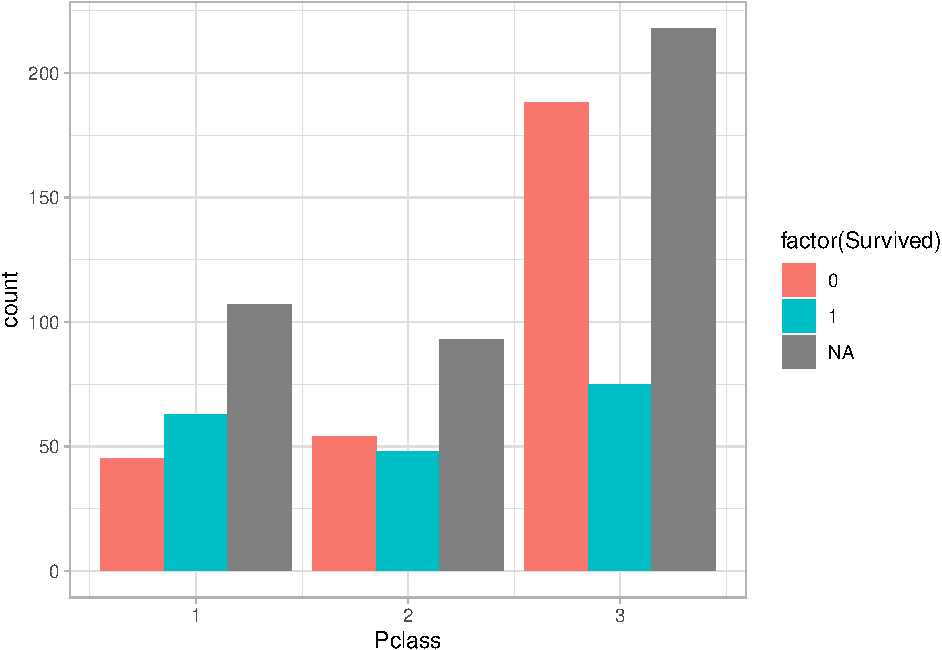
\includegraphics{final_pdf_files/figure-latex/unnamed-chunk-7-1.pdf}

\hypertarget{name}{%
\subsubsection{\texorpdfstring{\textbf{Name}}{Name}}\label{name}}

There were two people with the same name. The data shows that they were
different people.

\begin{Shaded}
\begin{Highlighting}[]
\FunctionTok{length}\NormalTok{(}\FunctionTok{unique}\NormalTok{(titanic\_full}\SpecialCharTok{$}\NormalTok{Name)) }\SpecialCharTok{\textless{}} \FunctionTok{nrow}\NormalTok{(titanic\_full)}
\end{Highlighting}
\end{Shaded}

\begin{verbatim}
## [1] TRUE
\end{verbatim}

\begin{Shaded}
\begin{Highlighting}[]
\NormalTok{titanic\_full }\SpecialCharTok{\%\textgreater{}\%}
  \FunctionTok{filter}\NormalTok{(Name }\SpecialCharTok{==} \StringTok{"Connolly, Miss. Kate"} \SpecialCharTok{|}\NormalTok{ Name }\SpecialCharTok{==} \StringTok{"Kelly, Mr. James"}\NormalTok{) }\SpecialCharTok{\%\textgreater{}\%}
  \FunctionTok{select}\NormalTok{(PassengerId, Survived, Name, Age, Ticket)}
\end{Highlighting}
\end{Shaded}

\begin{verbatim}
##   PassengerId Survived                 Name  Age Ticket
## 1         892       NA     Kelly, Mr. James 34.5 330911
## 2         898       NA Connolly, Miss. Kate 30.0 330972
## 3         290        1 Connolly, Miss. Kate 22.0 370373
## 4         697        0     Kelly, Mr. James 44.0 363592
\end{verbatim}

\hypertarget{sex}{%
\subsubsection{\texorpdfstring{\textbf{Sex}}{Sex}}\label{sex}}

\begin{Shaded}
\begin{Highlighting}[]
\FunctionTok{prop.table}\NormalTok{(}\FunctionTok{table}\NormalTok{(titanic\_full}\SpecialCharTok{$}\NormalTok{Sex))}
\end{Highlighting}
\end{Shaded}

\begin{verbatim}
## 
##    female      male 
## 0.3559969 0.6440031
\end{verbatim}

\hypertarget{age}{%
\subsubsection{\texorpdfstring{\textbf{Age}}{Age}}\label{age}}

Younger age passengers show higher survival rates. Age has quite a
problem with missing value. I will deal with this problem later.
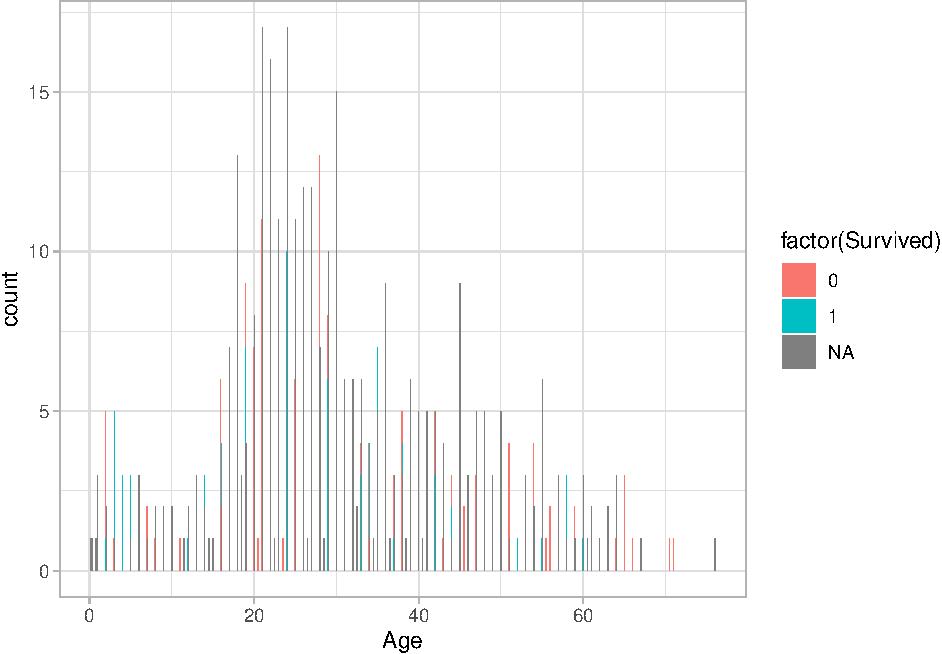
\includegraphics{final_pdf_files/figure-latex/unnamed-chunk-11-1.pdf}

\begin{Shaded}
\begin{Highlighting}[]
\FunctionTok{ggplot}\NormalTok{(titanic\_full, }\FunctionTok{aes}\NormalTok{(}\AttributeTok{x=}\NormalTok{titanic\_full}\SpecialCharTok{$}\NormalTok{Age, }\AttributeTok{y=}\NormalTok{titanic\_full}\SpecialCharTok{$}\NormalTok{Survived)) }\SpecialCharTok{+}
  \FunctionTok{geom\_point}\NormalTok{() }\SpecialCharTok{+}
  \FunctionTok{geom\_smooth}\NormalTok{(}\AttributeTok{method =}\NormalTok{ lm, }\AttributeTok{se=}\ConstantTok{TRUE}\NormalTok{)}
\end{Highlighting}
\end{Shaded}

\begin{verbatim}
## Warning: Use of `titanic_full$Age` is discouraged.
## i Use `Age` instead.
\end{verbatim}

\begin{verbatim}
## Warning: Use of `titanic_full$Survived` is discouraged.
## i Use `Survived` instead.
\end{verbatim}

\begin{verbatim}
## Warning: Use of `titanic_full$Age` is discouraged.
## i Use `Age` instead.
\end{verbatim}

\begin{verbatim}
## Warning: Use of `titanic_full$Survived` is discouraged.
## i Use `Survived` instead.
\end{verbatim}

\begin{verbatim}
## `geom_smooth()` using formula = 'y ~ x'
\end{verbatim}

\begin{verbatim}
## Warning: Removed 595 rows containing non-finite values (`stat_smooth()`).
\end{verbatim}

\begin{verbatim}
## Warning: Removed 595 rows containing missing values (`geom_point()`).
\end{verbatim}

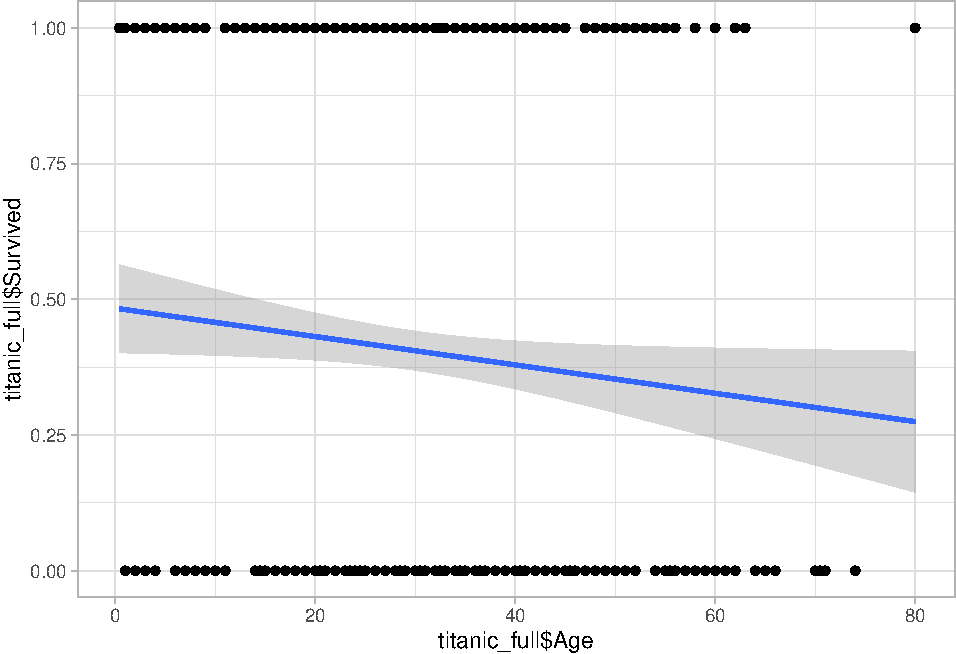
\includegraphics{final_pdf_files/figure-latex/unnamed-chunk-12-1.pdf}

\hypertarget{sibsp}{%
\subsubsection{\texorpdfstring{\textbf{SibSp}}{SibSp}}\label{sibsp}}

The number of siblings/spouse aboard the titanic. The mortality rate is
higher for those with fewer siblings and spouses.

\begin{Shaded}
\begin{Highlighting}[]
\FunctionTok{table}\NormalTok{(titanic\_full}\SpecialCharTok{$}\NormalTok{SibSp, titanic\_full}\SpecialCharTok{$}\NormalTok{Survived)}
\end{Highlighting}
\end{Shaded}

\begin{verbatim}
##    
##       0   1
##   0 398 210
##   1  97 112
##   2  15  13
##   3  12   4
##   4  15   3
##   5   5   0
##   8   7   0
\end{verbatim}

\begin{Shaded}
\begin{Highlighting}[]
\FunctionTok{prop.table}\NormalTok{(}\FunctionTok{table}\NormalTok{(titanic\_full}\SpecialCharTok{$}\NormalTok{SibSp, titanic\_full}\SpecialCharTok{$}\NormalTok{Survived), }\DecValTok{1}\NormalTok{)}
\end{Highlighting}
\end{Shaded}

\begin{verbatim}
##    
##             0         1
##   0 0.6546053 0.3453947
##   1 0.4641148 0.5358852
##   2 0.5357143 0.4642857
##   3 0.7500000 0.2500000
##   4 0.8333333 0.1666667
##   5 1.0000000 0.0000000
##   8 1.0000000 0.0000000
\end{verbatim}

\begin{Shaded}
\begin{Highlighting}[]
\FunctionTok{ggplot}\NormalTok{(titanic\_full[}\DecValTok{1}\SpecialCharTok{:}\DecValTok{891}\NormalTok{,],}\FunctionTok{aes}\NormalTok{(}\AttributeTok{x=}\NormalTok{SibSp, }\AttributeTok{fill=}\FunctionTok{factor}\NormalTok{(Survived))) }\SpecialCharTok{+}
  \FunctionTok{geom\_bar}\NormalTok{(}\AttributeTok{stat=}\StringTok{\textquotesingle{}count\textquotesingle{}}\NormalTok{, }\AttributeTok{position=}\StringTok{\textquotesingle{}dodge\textquotesingle{}}\NormalTok{)}
\end{Highlighting}
\end{Shaded}

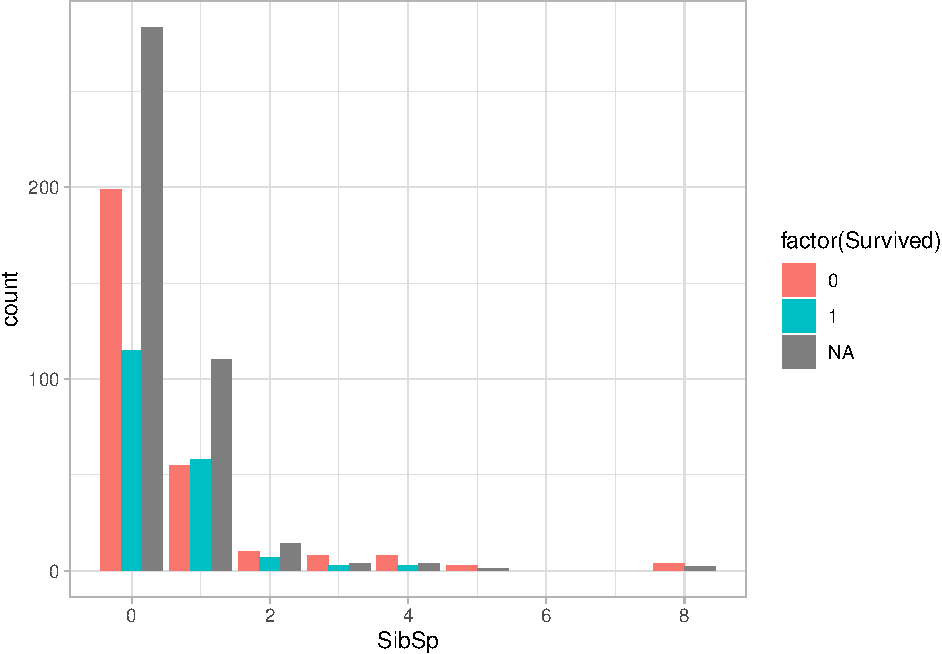
\includegraphics{final_pdf_files/figure-latex/unnamed-chunk-13-1.pdf}
\#\#\# \textbf{Parch} The number of parents/children aboard the titanic.
The mortality rate is higher when the number of parents and children is
smaller. Base on the visualization of SibSp and Parch, the family size
seems to be related to the survive. Therefore, I create the new variable
to indicate the family size.

\begin{Shaded}
\begin{Highlighting}[]
\FunctionTok{table}\NormalTok{(titanic\_full}\SpecialCharTok{$}\NormalTok{Parch, titanic\_full}\SpecialCharTok{$}\NormalTok{Survived)}
\end{Highlighting}
\end{Shaded}

\begin{verbatim}
##    
##       0   1
##   0 445 233
##   1  53  65
##   2  40  40
##   3   2   3
##   4   4   0
##   5   4   1
##   6   1   0
##   9   0   0
\end{verbatim}

\begin{Shaded}
\begin{Highlighting}[]
\FunctionTok{prop.table}\NormalTok{(}\FunctionTok{table}\NormalTok{(titanic\_full}\SpecialCharTok{$}\NormalTok{Parch, titanic\_full}\SpecialCharTok{$}\NormalTok{Survived))}
\end{Highlighting}
\end{Shaded}

\begin{verbatim}
##    
##               0           1
##   0 0.499438833 0.261503928
##   1 0.059483726 0.072951740
##   2 0.044893378 0.044893378
##   3 0.002244669 0.003367003
##   4 0.004489338 0.000000000
##   5 0.004489338 0.001122334
##   6 0.001122334 0.000000000
##   9 0.000000000 0.000000000
\end{verbatim}

\begin{Shaded}
\begin{Highlighting}[]
\FunctionTok{ggplot}\NormalTok{(titanic\_full[}\DecValTok{1}\SpecialCharTok{:}\DecValTok{891}\NormalTok{,],}\FunctionTok{aes}\NormalTok{(}\AttributeTok{x=}\NormalTok{Parch, }\AttributeTok{fill=}\FunctionTok{factor}\NormalTok{(Survived))) }\SpecialCharTok{+}
  \FunctionTok{geom\_bar}\NormalTok{(}\AttributeTok{stat=}\StringTok{\textquotesingle{}count\textquotesingle{}}\NormalTok{, }\AttributeTok{position=}\StringTok{\textquotesingle{}dodge\textquotesingle{}}\NormalTok{)}
\end{Highlighting}
\end{Shaded}

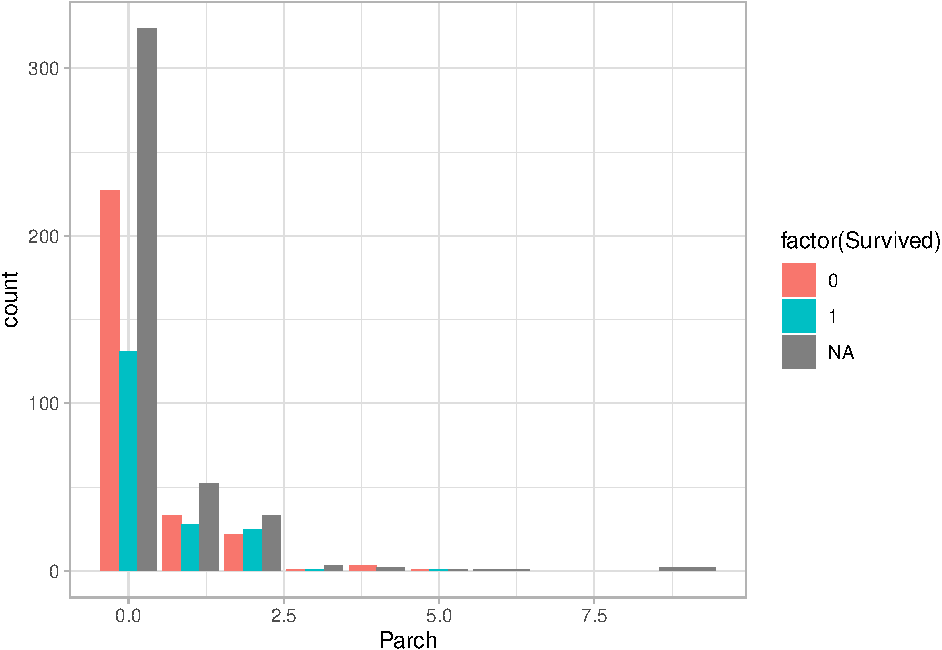
\includegraphics{final_pdf_files/figure-latex/unnamed-chunk-14-1.pdf}

Passengers with more family members are expected to have higher survival
rates, so a new variable was created to indicate the number of family
members.

\begin{Shaded}
\begin{Highlighting}[]
\CommentTok{\# The number of family member }
\NormalTok{titanic\_full}\SpecialCharTok{$}\NormalTok{Fsize }\OtherTok{\textless{}{-}}\NormalTok{ titanic\_full}\SpecialCharTok{$}\NormalTok{SibSp }\SpecialCharTok{+}\NormalTok{ titanic\_full}\SpecialCharTok{$}\NormalTok{Parch }\SpecialCharTok{+}\DecValTok{1}
\FunctionTok{table}\NormalTok{(titanic\_full}\SpecialCharTok{$}\NormalTok{Fsize, titanic\_full}\SpecialCharTok{$}\NormalTok{Survived)}
\end{Highlighting}
\end{Shaded}

\begin{verbatim}
##     
##        0   1
##   1  374 163
##   2   72  89
##   3   43  59
##   4    8  21
##   5   12   3
##   6   19   3
##   7    8   4
##   8    6   0
##   11   7   0
\end{verbatim}

\begin{Shaded}
\begin{Highlighting}[]
\FunctionTok{prop.table}\NormalTok{(}\FunctionTok{table}\NormalTok{(titanic\_full}\SpecialCharTok{$}\NormalTok{Fsize, titanic\_full}\SpecialCharTok{$}\NormalTok{Survived))}
\end{Highlighting}
\end{Shaded}

\begin{verbatim}
##     
##                0           1
##   1  0.419753086 0.182940516
##   2  0.080808081 0.099887767
##   3  0.048260382 0.066217733
##   4  0.008978676 0.023569024
##   5  0.013468013 0.003367003
##   6  0.021324355 0.003367003
##   7  0.008978676 0.004489338
##   8  0.006734007 0.000000000
##   11 0.007856341 0.000000000
\end{verbatim}

\begin{Shaded}
\begin{Highlighting}[]
\FunctionTok{ggplot}\NormalTok{(titanic\_full[}\DecValTok{1}\SpecialCharTok{:}\DecValTok{891}\NormalTok{,],}\FunctionTok{aes}\NormalTok{(}\AttributeTok{x=}\NormalTok{Fsize, }\AttributeTok{fill=}\FunctionTok{factor}\NormalTok{(Survived))) }\SpecialCharTok{+}
  \FunctionTok{geom\_bar}\NormalTok{(}\AttributeTok{stat=}\StringTok{\textquotesingle{}count\textquotesingle{}}\NormalTok{, }\AttributeTok{position=}\StringTok{\textquotesingle{}dodge\textquotesingle{}}\NormalTok{)}
\end{Highlighting}
\end{Shaded}

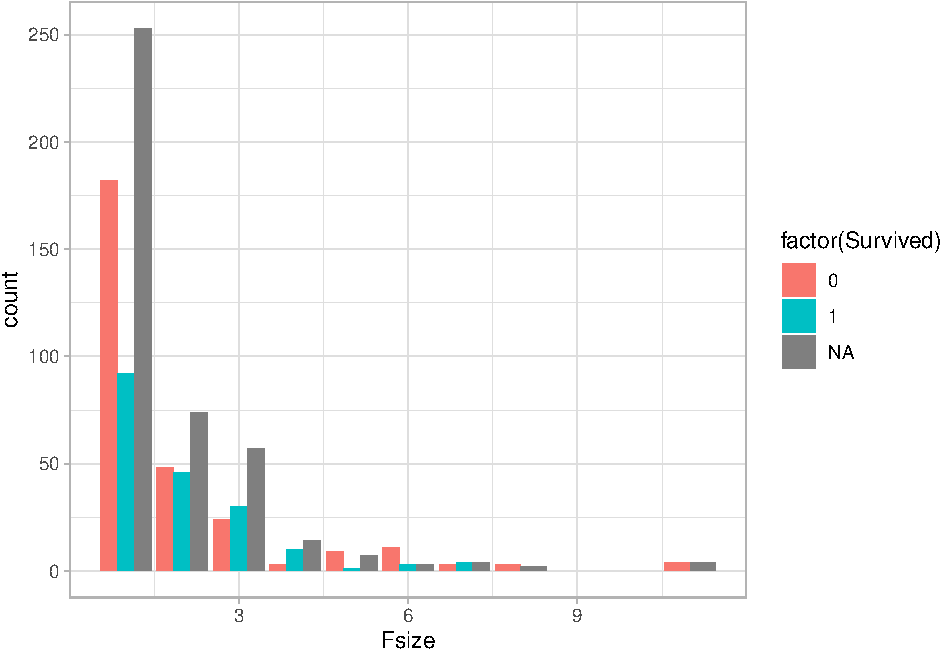
\includegraphics{final_pdf_files/figure-latex/unnamed-chunk-15-1.pdf}

\hypertarget{ticket}{%
\subsubsection{\texorpdfstring{\textbf{Ticket}}{Ticket}}\label{ticket}}

This is the Ticket number. Several passengers are fond to have the same
ticket number, This could mean that family members or others who rode
together may have shared tickets.

\begin{Shaded}
\begin{Highlighting}[]
\FunctionTok{length}\NormalTok{(}\FunctionTok{unique}\NormalTok{(titanic\_full}\SpecialCharTok{$}\NormalTok{Ticket))}
\end{Highlighting}
\end{Shaded}

\begin{verbatim}
## [1] 929
\end{verbatim}

\begin{Shaded}
\begin{Highlighting}[]
\NormalTok{titanic\_full }\SpecialCharTok{\%\textgreater{}\%}
  \FunctionTok{group\_by}\NormalTok{(Ticket) }\SpecialCharTok{\%\textgreater{}\%}
  \FunctionTok{count}\NormalTok{() }\SpecialCharTok{\%\textgreater{}\%}
  \FunctionTok{arrange}\NormalTok{(}\FunctionTok{desc}\NormalTok{(n))}
\end{Highlighting}
\end{Shaded}

\begin{verbatim}
## # A tibble: 929 x 2
## # Groups:   Ticket [929]
##    Ticket           n
##    <chr>        <int>
##  1 CA. 2343        11
##  2 1601             8
##  3 CA 2144          8
##  4 3101295          7
##  5 347077           7
##  6 347082           7
##  7 PC 17608         7
##  8 S.O.C. 14879     7
##  9 113781           6
## 10 19950            6
## # ... with 919 more rows
\end{verbatim}

\begin{Shaded}
\begin{Highlighting}[]
\NormalTok{titanic\_full }\SpecialCharTok{\%\textgreater{}\%}
  \FunctionTok{group\_by}\NormalTok{(Ticket, Fare) }\SpecialCharTok{\%\textgreater{}\%}
  \FunctionTok{count}\NormalTok{() }\SpecialCharTok{\%\textgreater{}\%}
  \FunctionTok{arrange}\NormalTok{(}\FunctionTok{desc}\NormalTok{(n))}
\end{Highlighting}
\end{Shaded}

\begin{verbatim}
## # A tibble: 930 x 3
## # Groups:   Ticket, Fare [930]
##    Ticket        Fare     n
##    <chr>        <dbl> <int>
##  1 CA. 2343      69.6    11
##  2 1601          56.5     8
##  3 CA 2144       46.9     8
##  4 3101295       39.7     7
##  5 347077        31.4     7
##  6 347082        31.3     7
##  7 PC 17608     262.      7
##  8 S.O.C. 14879  73.5     7
##  9 113781       152.      6
## 10 19950        263       6
## # ... with 920 more rows
\end{verbatim}

People with the same ticket have the same fare except the number 7534.

\begin{Shaded}
\begin{Highlighting}[]
\NormalTok{titanic\_full }\SpecialCharTok{\%\textgreater{}\%}
  \FunctionTok{filter}\NormalTok{(Ticket }\SpecialCharTok{==} \StringTok{\textquotesingle{}7534\textquotesingle{}}\NormalTok{)}
\end{Highlighting}
\end{Shaded}

\begin{verbatim}
##   PassengerId Pclass                          Name  Sex Age SibSp Parch Ticket
## 1         139      3           Osen, Mr. Olaf Elon male  16     0     0   7534
## 2         877      3 Gustafsson, Mr. Alfred Ossian male  20     0     0   7534
##     Fare Cabin Embarked Test_Data Survived Fsize
## 1 9.2167              S         1        0     1
## 2 9.8458              S         1        0     1
\end{verbatim}

\hypertarget{fare}{%
\subsubsection{\texorpdfstring{\textbf{Fare}}{Fare}}\label{fare}}

This is the passenger's fare. This shows a very right-skewed data and
there is one outliers at \textgreater500.

\begin{Shaded}
\begin{Highlighting}[]
\FunctionTok{ggplot}\NormalTok{(titanic\_full, }\FunctionTok{aes}\NormalTok{(}\AttributeTok{x =} \DecValTok{1}\NormalTok{, }\AttributeTok{y =}\NormalTok{ Fare)) }\SpecialCharTok{+} 
  \FunctionTok{geom\_boxplot}\NormalTok{() }\SpecialCharTok{+} 
  \FunctionTok{theme}\NormalTok{(}\AttributeTok{axis.ticks.y =} \FunctionTok{element\_blank}\NormalTok{(), }
        \AttributeTok{axis.text.y=}\FunctionTok{element\_blank}\NormalTok{(), }
        \AttributeTok{axis.title.y=}\FunctionTok{element\_blank}\NormalTok{()) }\SpecialCharTok{+} 
  \FunctionTok{scale\_y\_continuous}\NormalTok{(}\AttributeTok{breaks =} \FunctionTok{seq}\NormalTok{(}\DecValTok{0}\NormalTok{, }\DecValTok{600}\NormalTok{, }\DecValTok{50}\NormalTok{)) }\SpecialCharTok{+} 
  \FunctionTok{coord\_flip}\NormalTok{() }\SpecialCharTok{+} 
  \FunctionTok{ggtitle}\NormalTok{(}\StringTok{"Full Dataset {-} Fare"}\NormalTok{)}
\end{Highlighting}
\end{Shaded}

\begin{verbatim}
## Warning: Removed 1 rows containing non-finite values (`stat_boxplot()`).
\end{verbatim}

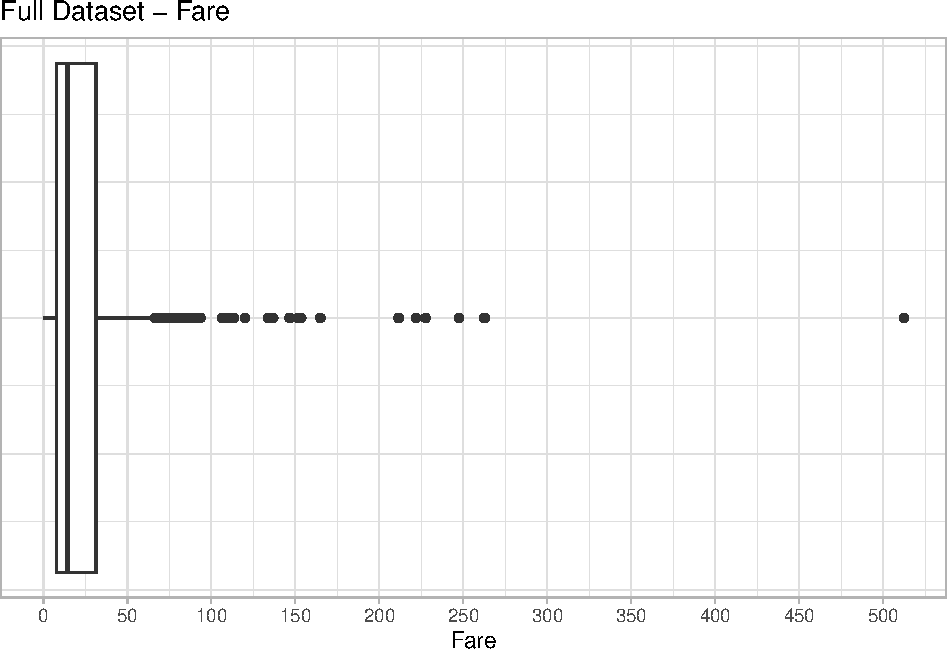
\includegraphics{final_pdf_files/figure-latex/unnamed-chunk-20-1.pdf}
After excluding outliers, the relationship between fares and survival
rates was examined and found that those who purchased more expensive
tickets had higher survival rates.

\begin{Shaded}
\begin{Highlighting}[]
\FunctionTok{ggplot}\NormalTok{(titanic\_full, }\FunctionTok{aes}\NormalTok{(}\AttributeTok{x =} \DecValTok{1}\NormalTok{, }\AttributeTok{y =}\NormalTok{ Fare)) }\SpecialCharTok{+} 
  \FunctionTok{geom\_boxplot}\NormalTok{() }\SpecialCharTok{+} 
  \FunctionTok{theme}\NormalTok{(}\AttributeTok{axis.ticks.y =} \FunctionTok{element\_blank}\NormalTok{(), }
        \AttributeTok{axis.text.y=}\FunctionTok{element\_blank}\NormalTok{(), }
        \AttributeTok{axis.title.y=}\FunctionTok{element\_blank}\NormalTok{()) }\SpecialCharTok{+} 
  \FunctionTok{scale\_y\_continuous}\NormalTok{(}\AttributeTok{limits =} \FunctionTok{c}\NormalTok{(}\DecValTok{0}\NormalTok{, }\DecValTok{300}\NormalTok{), }\AttributeTok{breaks =} \FunctionTok{seq}\NormalTok{(}\DecValTok{0}\NormalTok{, }\DecValTok{300}\NormalTok{, }\DecValTok{50}\NormalTok{)) }\SpecialCharTok{+} 
  \FunctionTok{facet\_grid}\NormalTok{(Survived }\SpecialCharTok{\textasciitilde{}}\NormalTok{ ., }\AttributeTok{labeller =}\NormalTok{ label\_both) }\SpecialCharTok{+} 
  \FunctionTok{coord\_flip}\NormalTok{() }\SpecialCharTok{+} 
  \FunctionTok{ggtitle}\NormalTok{(}\StringTok{"Full Dataset {-} Fare (Distributions, Survived vs Died)"}\NormalTok{)}
\end{Highlighting}
\end{Shaded}

\begin{verbatim}
## Warning: Removed 5 rows containing non-finite values (`stat_boxplot()`).
\end{verbatim}

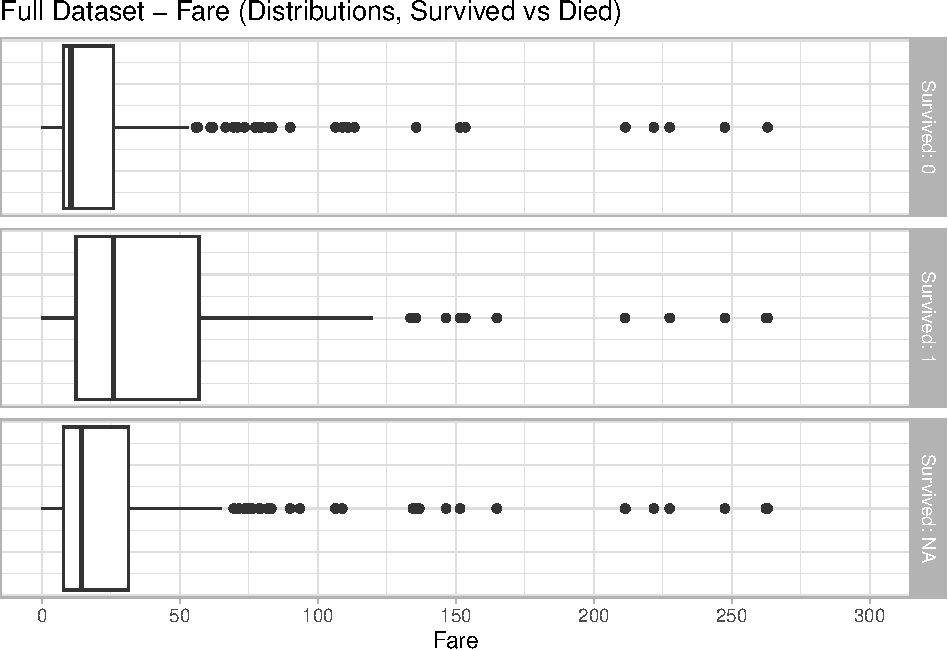
\includegraphics{final_pdf_files/figure-latex/unnamed-chunk-21-1.pdf}
\#\#\# \textbf{Cabin} The cabine number. There were lots of NA's

\begin{Shaded}
\begin{Highlighting}[]
\FunctionTok{sum}\NormalTok{(titanic\_full}\SpecialCharTok{$}\NormalTok{Cabin}\SpecialCharTok{==}\StringTok{""}\NormalTok{)}
\end{Highlighting}
\end{Shaded}

\begin{verbatim}
## [1] 1014
\end{verbatim}

It is possible to see certain trends in passengers whose Cabin' data is
missing.

\hypertarget{embarked}{%
\subsubsection{\texorpdfstring{\textbf{Embarked}}{Embarked}}\label{embarked}}

The port that the passenger embarked from (C = Cherbourg, Q =
Queenstown, S = Southampton). We can see that almost 70\% departed from
Southampton.

\begin{Shaded}
\begin{Highlighting}[]
\NormalTok{g11 }\OtherTok{\textless{}{-}}\NormalTok{ titanic\_full }\SpecialCharTok{\%\textgreater{}\%}
  \FunctionTok{filter}\NormalTok{(}\SpecialCharTok{!}\FunctionTok{is.na}\NormalTok{(Embarked)) }\SpecialCharTok{\%\textgreater{}\%}
\FunctionTok{ggplot}\NormalTok{(}\FunctionTok{aes}\NormalTok{(}\AttributeTok{x =} \FunctionTok{factor}\NormalTok{(Embarked))) }\SpecialCharTok{+} 
  \FunctionTok{geom\_bar}\NormalTok{(}\AttributeTok{fill =} \StringTok{"deepskyblue4"}\NormalTok{) }\SpecialCharTok{+} 
  \FunctionTok{scale\_y\_continuous}\NormalTok{(}\AttributeTok{breaks =} \FunctionTok{seq}\NormalTok{(}\DecValTok{0}\NormalTok{, }\DecValTok{1000}\NormalTok{, }\DecValTok{100}\NormalTok{)) }\SpecialCharTok{+} 
  \FunctionTok{labs}\NormalTok{(}\AttributeTok{x =} \StringTok{"Embarked"}\NormalTok{, }\AttributeTok{y =} \StringTok{"Count"}\NormalTok{) }\SpecialCharTok{+} 
  \FunctionTok{ggtitle}\NormalTok{(}\StringTok{"Full Dataset {-} Embarked"}\NormalTok{) }\SpecialCharTok{+}
  \FunctionTok{theme}\NormalTok{(}\AttributeTok{plot.title =} \FunctionTok{element\_text}\NormalTok{(}\AttributeTok{size =} \DecValTok{10}\NormalTok{, }\AttributeTok{face =} \StringTok{"bold"}\NormalTok{))}


\NormalTok{g12 }\OtherTok{\textless{}{-}}\NormalTok{ train\_titanic }\SpecialCharTok{\%\textgreater{}\%}
  \FunctionTok{filter}\NormalTok{(}\SpecialCharTok{!}\FunctionTok{is.na}\NormalTok{(Embarked)) }\SpecialCharTok{\%\textgreater{}\%}
\FunctionTok{ggplot}\NormalTok{(}\FunctionTok{aes}\NormalTok{(}\AttributeTok{x =} \FunctionTok{factor}\NormalTok{(Embarked), }\AttributeTok{fill =} \FunctionTok{factor}\NormalTok{(Survived))) }\SpecialCharTok{+} 
  \FunctionTok{geom\_bar}\NormalTok{(}\AttributeTok{fill =} \StringTok{"darkgreen"}\NormalTok{) }\SpecialCharTok{+} 
  \FunctionTok{scale\_y\_continuous}\NormalTok{(}\AttributeTok{breaks =} \FunctionTok{seq}\NormalTok{(}\DecValTok{0}\NormalTok{, }\DecValTok{500}\NormalTok{, }\DecValTok{50}\NormalTok{)) }\SpecialCharTok{+} 
  \FunctionTok{scale\_fill\_discrete}\NormalTok{(}\AttributeTok{name =} \StringTok{"Survived"}\NormalTok{) }\SpecialCharTok{+}
  \FunctionTok{labs}\NormalTok{(}\AttributeTok{x =} \StringTok{"Embarked"}\NormalTok{, }\AttributeTok{y =} \StringTok{"Count"}\NormalTok{) }\SpecialCharTok{+} 
  \FunctionTok{ggtitle}\NormalTok{(}\StringTok{"Train Dataset {-} Embarked (Proportion Survived)"}\NormalTok{) }

\NormalTok{g11}
\end{Highlighting}
\end{Shaded}

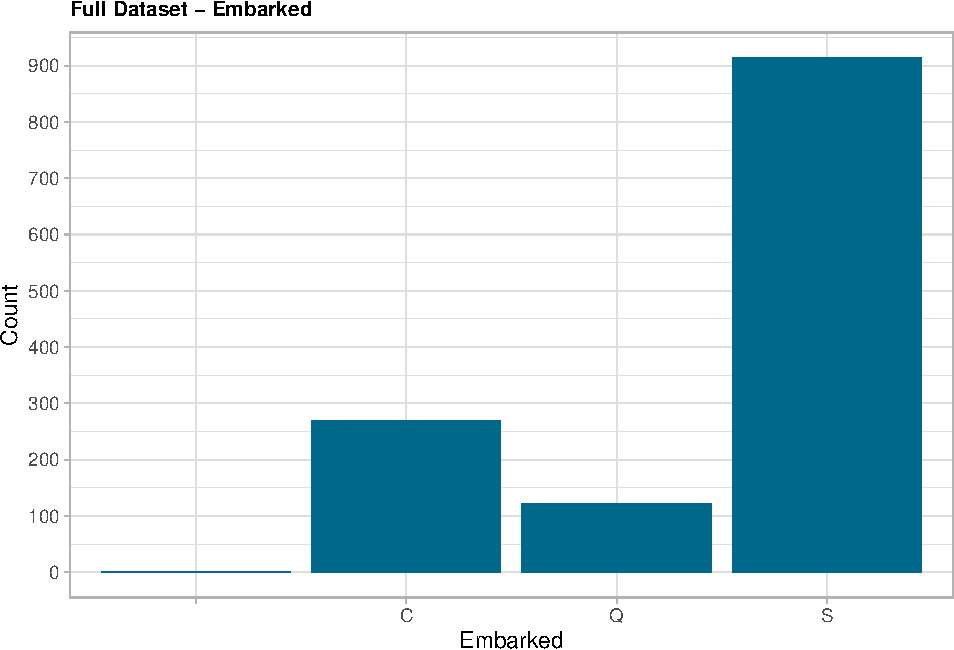
\includegraphics{final_pdf_files/figure-latex/unnamed-chunk-23-1.pdf}

\begin{Shaded}
\begin{Highlighting}[]
\NormalTok{g12}
\end{Highlighting}
\end{Shaded}

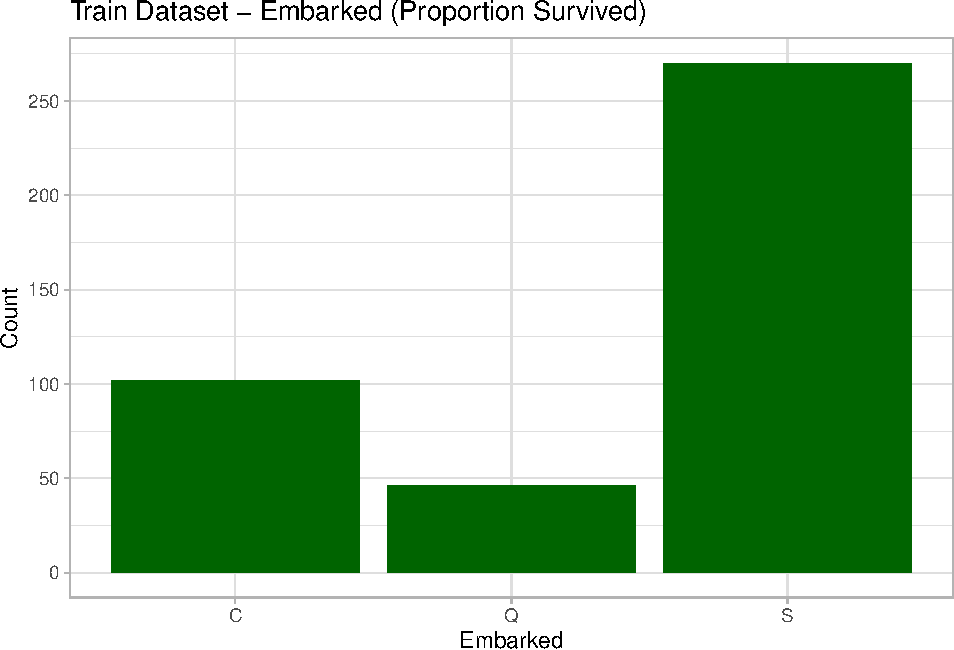
\includegraphics{final_pdf_files/figure-latex/unnamed-chunk-23-2.pdf}

\hypertarget{feature-engineering-missing-value-imputation}{%
\section{\texorpdfstring{\textbf{3. Feature Engineering \$ Missing Value
Imputation}}{3. Feature Engineering \$ Missing Value Imputation}}\label{feature-engineering-missing-value-imputation}}

\hypertarget{feature-engineering}{%
\subsection{\texorpdfstring{\textbf{3.1 Feature
Engineering}}{3.1 Feature Engineering}}\label{feature-engineering}}

\hypertarget{title}{%
\subsubsection{\texorpdfstring{\textbf{3.1.1
Title}}{3.1.1 Title}}\label{title}}

From the evaluation of the variables so far, I have found that survival
rates are higher for economically well-off individuals and for women.
Thus, it is possible that survival rates can be predicted from name
titles. I subtracted the Title from \emph{Name} by using regular
expression.

\begin{Shaded}
\begin{Highlighting}[]
\NormalTok{titanic\_full}\SpecialCharTok{$}\NormalTok{Title }\OtherTok{\textless{}{-}} \FunctionTok{gsub}\NormalTok{(}\StringTok{\textquotesingle{}(.*, )|(}\SpecialCharTok{\textbackslash{}\textbackslash{}}\StringTok{..*)\textquotesingle{}}\NormalTok{, }\StringTok{\textquotesingle{}\textquotesingle{}}\NormalTok{, titanic\_full}\SpecialCharTok{$}\NormalTok{Name)}
\NormalTok{titanic\_full}\SpecialCharTok{$}\NormalTok{Surname }\OtherTok{\textless{}{-}} \FunctionTok{sapply}\NormalTok{(titanic\_full}\SpecialCharTok{$}\NormalTok{Name, }\ControlFlowTok{function}\NormalTok{(x) }\FunctionTok{strsplit}\NormalTok{(x, }\AttributeTok{split =} \StringTok{\textquotesingle{}[,.]\textquotesingle{}}\NormalTok{)[[}\DecValTok{1}\NormalTok{]][}\DecValTok{1}\NormalTok{])}
\FunctionTok{table}\NormalTok{(titanic\_full}\SpecialCharTok{$}\NormalTok{Title, titanic\_full}\SpecialCharTok{$}\NormalTok{Survived)}
\end{Highlighting}
\end{Shaded}

\begin{verbatim}
##               
##                  0   1
##   Capt           1   0
##   Col            1   1
##   Don            1   0
##   Dona           0   0
##   Dr             4   3
##   Jonkheer       1   0
##   Lady           0   1
##   Major          1   1
##   Master        17  23
##   Miss          55 127
##   Mlle           0   2
##   Mme            0   1
##   Mr           436  81
##   Mrs           26  99
##   Ms             0   1
##   Rev            6   0
##   Sir            0   1
##   the Countess   0   1
\end{verbatim}

\begin{Shaded}
\begin{Highlighting}[]
\FunctionTok{table}\NormalTok{(titanic\_full}\SpecialCharTok{$}\NormalTok{Sex, titanic\_full}\SpecialCharTok{$}\NormalTok{Title)}
\end{Highlighting}
\end{Shaded}

\begin{verbatim}
##         
##          Capt Col Don Dona  Dr Jonkheer Lady Major Master Miss Mlle Mme  Mr Mrs
##   female    0   0   0    1   1        0    1     0      0  260    2   1   0 197
##   male      1   4   1    0   7        1    0     2     61    0    0   0 757   0
##         
##           Ms Rev Sir the Countess
##   female   2   0   0            1
##   male     0   8   1            0
\end{verbatim}

\begin{Shaded}
\begin{Highlighting}[]
\FunctionTok{prop.table}\NormalTok{(}\FunctionTok{table}\NormalTok{(titanic\_full}\SpecialCharTok{$}\NormalTok{Title, titanic\_full}\SpecialCharTok{$}\NormalTok{Survived), }\DecValTok{1}\NormalTok{)}
\end{Highlighting}
\end{Shaded}

\begin{verbatim}
##               
##                        0         1
##   Capt         1.0000000 0.0000000
##   Col          0.5000000 0.5000000
##   Don          1.0000000 0.0000000
##   Dona                            
##   Dr           0.5714286 0.4285714
##   Jonkheer     1.0000000 0.0000000
##   Lady         0.0000000 1.0000000
##   Major        0.5000000 0.5000000
##   Master       0.4250000 0.5750000
##   Miss         0.3021978 0.6978022
##   Mlle         0.0000000 1.0000000
##   Mme          0.0000000 1.0000000
##   Mr           0.8433269 0.1566731
##   Mrs          0.2080000 0.7920000
##   Ms           0.0000000 1.0000000
##   Rev          1.0000000 0.0000000
##   Sir          0.0000000 1.0000000
##   the Countess 0.0000000 1.0000000
\end{verbatim}

\begin{Shaded}
\begin{Highlighting}[]
\FunctionTok{ggplot}\NormalTok{(titanic\_full[}\DecValTok{1}\SpecialCharTok{:}\DecValTok{891}\NormalTok{, ], }\FunctionTok{aes}\NormalTok{(}\AttributeTok{x =}\NormalTok{ Title, }\AttributeTok{fill =} \FunctionTok{factor}\NormalTok{(Survived))) }\SpecialCharTok{+} 
  \FunctionTok{geom\_bar}\NormalTok{(}\AttributeTok{stat=}\StringTok{\textquotesingle{}count\textquotesingle{}}\NormalTok{, }\AttributeTok{position=}\StringTok{\textquotesingle{}dodge\textquotesingle{}}\NormalTok{) }
\end{Highlighting}
\end{Shaded}

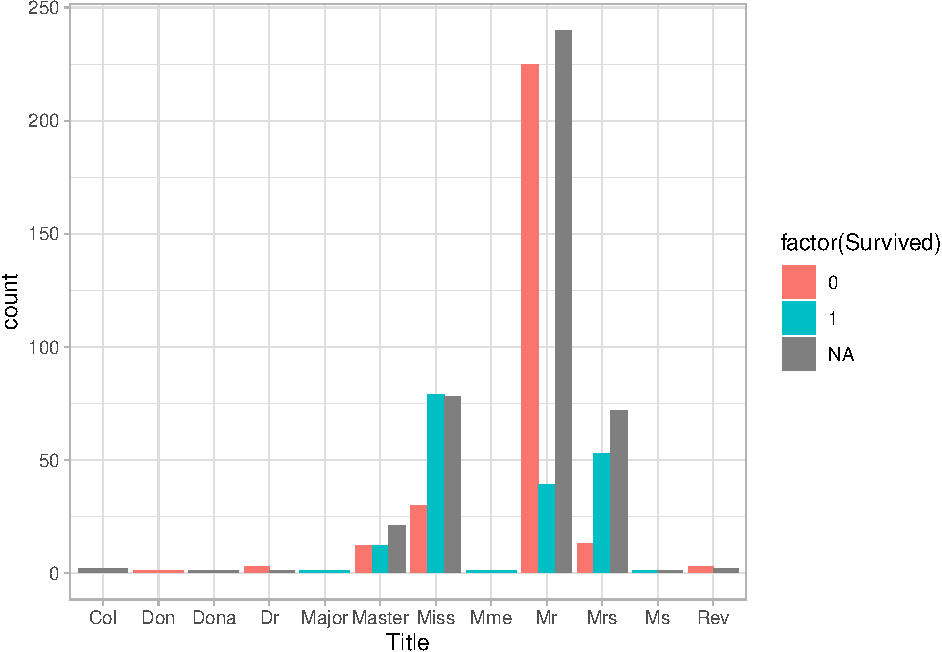
\includegraphics{final_pdf_files/figure-latex/unnamed-chunk-25-1.pdf}
There are several few titles. We have summarized and categorized them
into groups of six titles.

\begin{Shaded}
\begin{Highlighting}[]
\NormalTok{officer }\OtherTok{\textless{}{-}} \FunctionTok{c}\NormalTok{(}\StringTok{\textquotesingle{}Capt\textquotesingle{}}\NormalTok{, }\StringTok{\textquotesingle{}Col\textquotesingle{}}\NormalTok{, }\StringTok{\textquotesingle{}Don\textquotesingle{}}\NormalTok{, }\StringTok{\textquotesingle{}Dr\textquotesingle{}}\NormalTok{, }\StringTok{\textquotesingle{}Major\textquotesingle{}}\NormalTok{, }\StringTok{\textquotesingle{}Rev\textquotesingle{}}\NormalTok{)}
\NormalTok{royalty }\OtherTok{\textless{}{-}} \FunctionTok{c}\NormalTok{(}\StringTok{\textquotesingle{}Dona\textquotesingle{}}\NormalTok{, }\StringTok{\textquotesingle{}Lady\textquotesingle{}}\NormalTok{, }\StringTok{\textquotesingle{}the Countess\textquotesingle{}}\NormalTok{, }\StringTok{\textquotesingle{}Sir\textquotesingle{}}\NormalTok{, }\StringTok{\textquotesingle{}Jonkheer\textquotesingle{}}\NormalTok{)}
\NormalTok{titanic\_full}\SpecialCharTok{$}\NormalTok{Title[titanic\_full}\SpecialCharTok{$}\NormalTok{Title }\SpecialCharTok{==} \StringTok{\textquotesingle{}Mlle\textquotesingle{}}\NormalTok{] }\OtherTok{\textless{}{-}} \StringTok{\textquotesingle{}Miss\textquotesingle{}}
\NormalTok{titanic\_full}\SpecialCharTok{$}\NormalTok{Title[titanic\_full}\SpecialCharTok{$}\NormalTok{Title }\SpecialCharTok{==} \StringTok{\textquotesingle{}Ms\textquotesingle{}}\NormalTok{] }\OtherTok{\textless{}{-}} \StringTok{\textquotesingle{}Miss\textquotesingle{}}
\NormalTok{titanic\_full}\SpecialCharTok{$}\NormalTok{Title[titanic\_full}\SpecialCharTok{$}\NormalTok{Title }\SpecialCharTok{==} \StringTok{\textquotesingle{}Mme\textquotesingle{}}\NormalTok{] }\OtherTok{\textless{}{-}} \StringTok{\textquotesingle{}Mrs\textquotesingle{}}
\NormalTok{titanic\_full}\SpecialCharTok{$}\NormalTok{Title[titanic\_full}\SpecialCharTok{$}\NormalTok{Title }\SpecialCharTok{\%in\%}\NormalTok{ royalty] }\OtherTok{\textless{}{-}} \StringTok{\textquotesingle{}Royalty\textquotesingle{}}
\NormalTok{titanic\_full}\SpecialCharTok{$}\NormalTok{Title[titanic\_full}\SpecialCharTok{$}\NormalTok{Title }\SpecialCharTok{\%in\%}\NormalTok{ officer] }\OtherTok{\textless{}{-}} \StringTok{\textquotesingle{}Officer\textquotesingle{}}
\NormalTok{titanic\_full}\SpecialCharTok{$}\NormalTok{Title }\OtherTok{=} \FunctionTok{as.factor}\NormalTok{(titanic\_full}\SpecialCharTok{$}\NormalTok{Title)}
\end{Highlighting}
\end{Shaded}

\begin{Shaded}
\begin{Highlighting}[]
\FunctionTok{ggplot}\NormalTok{(titanic\_full[}\DecValTok{1}\SpecialCharTok{:}\DecValTok{891}\NormalTok{,],}\FunctionTok{aes}\NormalTok{(}\AttributeTok{x=}\NormalTok{Title, }\AttributeTok{fill=}\FunctionTok{factor}\NormalTok{(Survived))) }\SpecialCharTok{+}
  \FunctionTok{geom\_bar}\NormalTok{(}\AttributeTok{stat=}\StringTok{\textquotesingle{}count\textquotesingle{}}\NormalTok{, }\AttributeTok{position=}\StringTok{\textquotesingle{}dodge\textquotesingle{}}\NormalTok{) }
\end{Highlighting}
\end{Shaded}

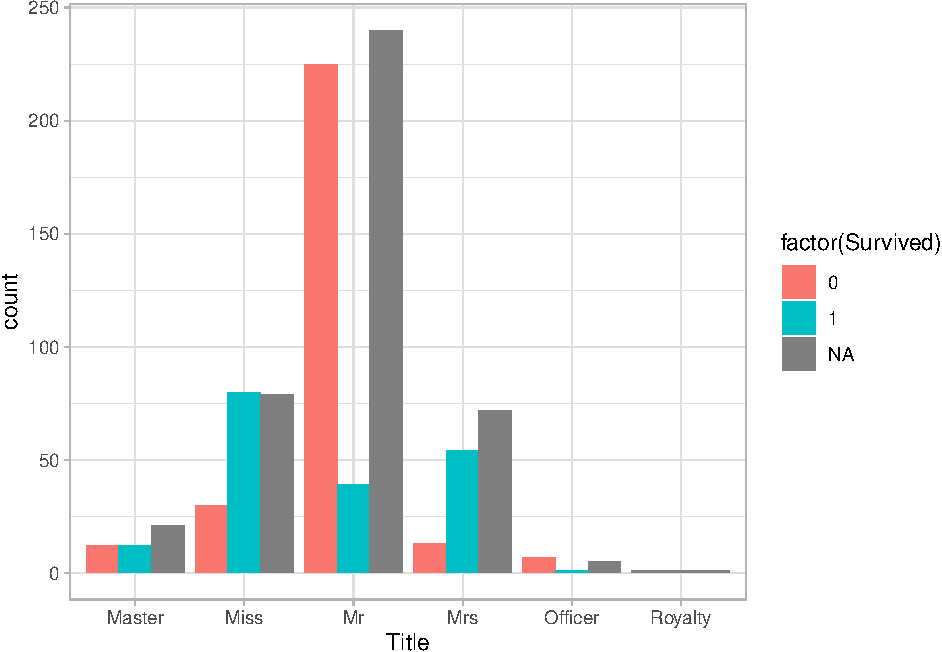
\includegraphics{final_pdf_files/figure-latex/unnamed-chunk-27-1.pdf} It
can be seen that the mortality rate is very high for those with the
title ``Mr.''.

\hypertarget{cabin-data}{%
\subsubsection{\texorpdfstring{\textbf{3.1.2 Cabin
data}}{3.1.2 Cabin data}}\label{cabin-data}}

Many part of cabin data was missing. Since assigning missing values
would place a very strong presumption, I made it a binary variable with
and without data.

\begin{Shaded}
\begin{Highlighting}[]
\NormalTok{titanic\_full}\SpecialCharTok{$}\NormalTok{Cabin\_dat }\OtherTok{\textless{}{-}} \FunctionTok{ifelse}\NormalTok{(}\SpecialCharTok{!}\NormalTok{(titanic\_full}\SpecialCharTok{$}\NormalTok{Cabin}\SpecialCharTok{==}\StringTok{""}\NormalTok{), }\DecValTok{1}\NormalTok{, }\DecValTok{0}\NormalTok{)}
\FunctionTok{prop.table}\NormalTok{(}\FunctionTok{table}\NormalTok{(titanic\_full}\SpecialCharTok{$}\NormalTok{Cabin\_dat))}
\end{Highlighting}
\end{Shaded}

\begin{verbatim}
## 
##         0         1 
## 0.7746371 0.2253629
\end{verbatim}

\hypertarget{fare-per-person}{%
\subsubsection{\texorpdfstring{\textbf{3.1.3 Fare (per
person)}}{3.1.3 Fare (per person)}}\label{fare-per-person}}

We created the per capita fare cost as a variable because it is possible
that more affluent people purchase more expensive tickets and have
higher survival rates.

\begin{Shaded}
\begin{Highlighting}[]
\NormalTok{fare\_pp }\OtherTok{\textless{}{-}}\NormalTok{ titanic\_full }\SpecialCharTok{\%\textgreater{}\%}
  \FunctionTok{group\_by}\NormalTok{(Ticket, Fare) }\SpecialCharTok{\%\textgreater{}\%}
  \FunctionTok{summarise}\NormalTok{(}\AttributeTok{Group\_size\_FE =} \FunctionTok{n}\NormalTok{()) }\SpecialCharTok{\%\textgreater{}\%}
  \FunctionTok{mutate}\NormalTok{(}\AttributeTok{Fare\_pp\_FE =}\NormalTok{ Fare }\SpecialCharTok{/}\NormalTok{ Group\_size\_FE)}
\end{Highlighting}
\end{Shaded}

\begin{verbatim}
## `summarise()` has grouped output by 'Ticket'. You can override using the
## `.groups` argument.
\end{verbatim}

\begin{Shaded}
\begin{Highlighting}[]
\NormalTok{titanic\_full }\OtherTok{\textless{}{-}} \FunctionTok{left\_join}\NormalTok{(titanic\_full, fare\_pp, }\AttributeTok{by=}\FunctionTok{c}\NormalTok{(}\StringTok{"Ticket"}\NormalTok{, }\StringTok{"Fare"}\NormalTok{))}
\end{Highlighting}
\end{Shaded}

\begin{Shaded}
\begin{Highlighting}[]
\NormalTok{g13 }\OtherTok{\textless{}{-}} \FunctionTok{ggplot}\NormalTok{(titanic\_full, }\FunctionTok{aes}\NormalTok{(}\AttributeTok{x =}\NormalTok{ Group\_size\_FE, }\AttributeTok{y =}\NormalTok{ Fare)) }\SpecialCharTok{+} 
  \FunctionTok{geom\_jitter}\NormalTok{(}\AttributeTok{alpha =} \FloatTok{0.2}\NormalTok{) }\SpecialCharTok{+} 
  \FunctionTok{geom\_smooth}\NormalTok{(}\AttributeTok{method =} \StringTok{"lm"}\NormalTok{, }\AttributeTok{se =}\NormalTok{ F) }\SpecialCharTok{+} 
  \FunctionTok{scale\_y\_continuous}\NormalTok{(}\AttributeTok{limits =} \FunctionTok{c}\NormalTok{(}\DecValTok{0}\NormalTok{, }\DecValTok{300}\NormalTok{)) }\SpecialCharTok{+} 
  \FunctionTok{labs}\NormalTok{(}\AttributeTok{x =} \StringTok{"Group Size"}\NormalTok{, }\AttributeTok{y =} \StringTok{"Fare"}\NormalTok{) }\SpecialCharTok{+} 
  \FunctionTok{theme}\NormalTok{(}\AttributeTok{legend.position =} \StringTok{"none"}\NormalTok{)}

\NormalTok{g14 }\OtherTok{\textless{}{-}} \FunctionTok{ggplot}\NormalTok{(titanic\_full, }\FunctionTok{aes}\NormalTok{(}\AttributeTok{x =}\NormalTok{ Group\_size\_FE, }\AttributeTok{y =}\NormalTok{ Fare, }\AttributeTok{col =} \FunctionTok{factor}\NormalTok{(Pclass))) }\SpecialCharTok{+} 
  \FunctionTok{geom\_jitter}\NormalTok{(}\AttributeTok{alpha =} \FloatTok{0.2}\NormalTok{) }\SpecialCharTok{+} 
  \FunctionTok{geom\_smooth}\NormalTok{(}\AttributeTok{method =} \StringTok{"lm"}\NormalTok{, }\AttributeTok{se =}\NormalTok{ F) }\SpecialCharTok{+} 
  \FunctionTok{facet\_grid}\NormalTok{(Pclass }\SpecialCharTok{\textasciitilde{}}\NormalTok{ ., }\AttributeTok{labeller =}\NormalTok{ label\_both) }\SpecialCharTok{+} 
  \FunctionTok{scale\_y\_continuous}\NormalTok{(}\AttributeTok{limits =} \FunctionTok{c}\NormalTok{(}\DecValTok{0}\NormalTok{, }\DecValTok{300}\NormalTok{)) }\SpecialCharTok{+} 
  \FunctionTok{labs}\NormalTok{(}\AttributeTok{x =} \StringTok{"Group Size"}\NormalTok{, }\AttributeTok{y =} \StringTok{"Fare"}\NormalTok{) }\SpecialCharTok{+} 
  \FunctionTok{theme}\NormalTok{(}\AttributeTok{legend.position =} \StringTok{"none"}\NormalTok{)}

\FunctionTok{grid.arrange}\NormalTok{(g13, g14, }\AttributeTok{ncol =} \DecValTok{2}\NormalTok{)}
\end{Highlighting}
\end{Shaded}

\begin{verbatim}
## `geom_smooth()` using formula = 'y ~ x'
\end{verbatim}

\begin{verbatim}
## Warning: Removed 5 rows containing non-finite values (`stat_smooth()`).
\end{verbatim}

\begin{verbatim}
## Warning: Removed 10 rows containing missing values (`geom_point()`).
\end{verbatim}

\begin{verbatim}
## `geom_smooth()` using formula = 'y ~ x'
\end{verbatim}

\begin{verbatim}
## Warning: Removed 5 rows containing non-finite values (`stat_smooth()`).
\end{verbatim}

\begin{verbatim}
## Warning: Removed 11 rows containing missing values (`geom_point()`).
\end{verbatim}

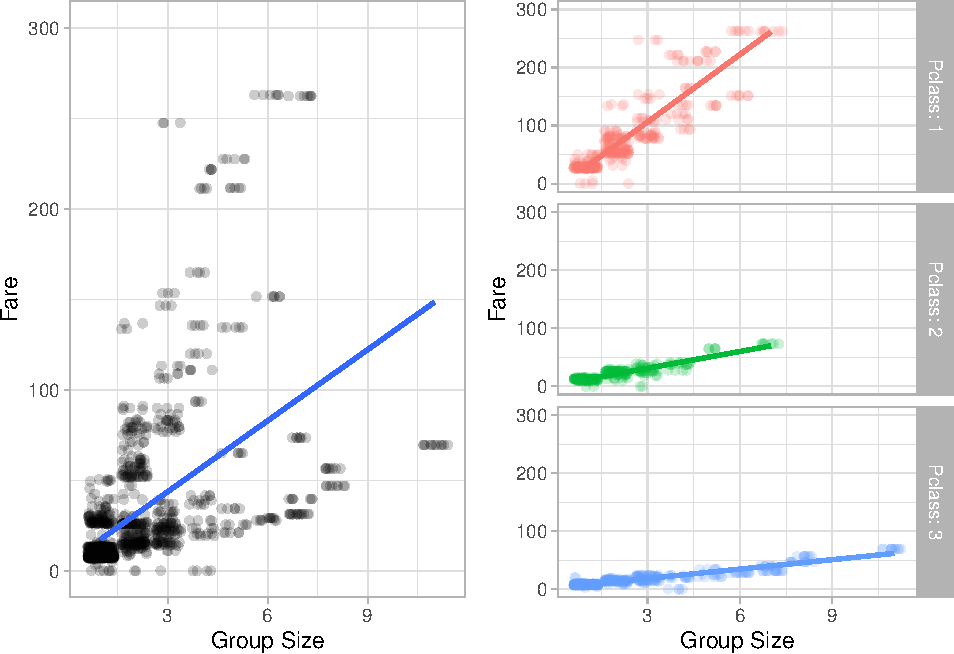
\includegraphics{final_pdf_files/figure-latex/unnamed-chunk-31-1.pdf}
There are correlation between Group size and Pclass. \#\#\#
\textbf{3.1.4} Based on previous studies, it is possible that the larger
the family size, the higher the survival rate. Thus, I created a family
size variable.

\begin{Shaded}
\begin{Highlighting}[]
\NormalTok{titanic\_full}\SpecialCharTok{$}\NormalTok{Family\_size\_FE }\OtherTok{\textless{}{-}}\NormalTok{ titanic\_full}\SpecialCharTok{$}\NormalTok{SibSp }\SpecialCharTok{+}\NormalTok{ titanic\_full}\SpecialCharTok{$}\NormalTok{Parch }\SpecialCharTok{+} \DecValTok{1}

\NormalTok{titanic\_full}\SpecialCharTok{$}\NormalTok{Total\_group\_size\_FE }\OtherTok{\textless{}{-}} \FunctionTok{pmax}\NormalTok{(titanic\_full}\SpecialCharTok{$}\NormalTok{Family\_size\_FE, titanic\_full}\SpecialCharTok{$}\NormalTok{Group\_size\_FE)}
\end{Highlighting}
\end{Shaded}

\hypertarget{missing-value}{%
\subsection{\texorpdfstring{\textbf{3.2 Missing
Value}}{3.2 Missing Value}}\label{missing-value}}

From here, I have addressed the variables with missing values. I know
that there were missing values in \textbf{Age}, and
\textbf{Fare\_pp\_FE}. I also know that \textbf{Embarked} has a blank
entry.

\begin{Shaded}
\begin{Highlighting}[]
\NormalTok{titanic\_full }\OtherTok{\textless{}{-}}\NormalTok{ titanic\_full }\SpecialCharTok{\%\textgreater{}\%}
  \FunctionTok{select}\NormalTok{(}\SpecialCharTok{{-}}\FunctionTok{c}\NormalTok{(Name, Ticket, Cabin, Group\_size\_FE, Fare))}

\FunctionTok{missing\_vars}\NormalTok{(titanic\_full)}
\end{Highlighting}
\end{Shaded}

\begin{verbatim}
##                    var missing missing_prop
## 1             Survived     418 0.3193277311
## 2                  Age     263 0.2009167303
## 3           Fare_pp_FE       1 0.0007639419
## 4          PassengerId       0 0.0000000000
## 5               Pclass       0 0.0000000000
## 6                  Sex       0 0.0000000000
## 7                SibSp       0 0.0000000000
## 8                Parch       0 0.0000000000
## 9             Embarked       0 0.0000000000
## 10           Test_Data       0 0.0000000000
## 11               Fsize       0 0.0000000000
## 12               Title       0 0.0000000000
## 13             Surname       0 0.0000000000
## 14           Cabin_dat       0 0.0000000000
## 15      Family_size_FE       0 0.0000000000
## 16 Total_group_size_FE       0 0.0000000000
\end{verbatim}

\hypertarget{fare-1}{%
\subsubsection{\texorpdfstring{\textbf{3.2.1
Fare}}{3.2.1 Fare}}\label{fare-1}}

\begin{Shaded}
\begin{Highlighting}[]
\NormalTok{titanic\_full[}\FunctionTok{is.na}\NormalTok{(titanic\_full}\SpecialCharTok{$}\NormalTok{Fare\_pp\_FE), ]}
\end{Highlighting}
\end{Shaded}

\begin{verbatim}
##     PassengerId Pclass  Sex  Age SibSp Parch Embarked Test_Data Survived Fsize
## 153        1044      3 male 60.5     0     0        S         0       NA     1
##     Title Surname Cabin_dat Fare_pp_FE Family_size_FE Total_group_size_FE
## 153    Mr  Storey         0         NA              1                   1
\end{verbatim}

There was only one missing value. Since there was one missing value, the
median value was assigned instead of taking a special imputation method
to save time.

\begin{Shaded}
\begin{Highlighting}[]
\NormalTok{titanic\_full}\SpecialCharTok{$}\NormalTok{Fare\_pp\_FE[}\FunctionTok{is.na}\NormalTok{(titanic\_full}\SpecialCharTok{$}\NormalTok{Fare\_pp\_FE)] }\OtherTok{\textless{}{-}} \FunctionTok{median}\NormalTok{(titanic\_full}\SpecialCharTok{$}\NormalTok{Fare\_pp\_FE, }\AttributeTok{na.rm =}\NormalTok{ T)}
\end{Highlighting}
\end{Shaded}

\hypertarget{embarked-1}{%
\subsubsection{\texorpdfstring{\textbf{3.2.2
Embarked}}{3.2.2 Embarked}}\label{embarked-1}}

I can see that there are two missing calues in the \textbf{Embarked}.
Most passengers are classified as ``S''. However, they are classified as
``C'' because their ticket price is high and it is possible that the
wealthier passengers are from ``C''.

\begin{Shaded}
\begin{Highlighting}[]
\FunctionTok{which}\NormalTok{(titanic\_full}\SpecialCharTok{$}\NormalTok{Embarked }\SpecialCharTok{==} \StringTok{""}\NormalTok{)}
\end{Highlighting}
\end{Shaded}

\begin{verbatim}
## [1]  480 1248
\end{verbatim}

\begin{Shaded}
\begin{Highlighting}[]
\NormalTok{titanic\_full[}\FunctionTok{c}\NormalTok{(}\DecValTok{480}\NormalTok{, }\DecValTok{1248}\NormalTok{), ]}
\end{Highlighting}
\end{Shaded}

\begin{verbatim}
##      PassengerId Pclass    Sex Age SibSp Parch Embarked Test_Data Survived
## 480           62      1 female  38     0     0                  1        1
## 1248         830      1 female  62     0     0                  1        1
##      Fsize Title Surname Cabin_dat Fare_pp_FE Family_size_FE
## 480      1  Miss   Icard         1         40              1
## 1248     1   Mrs   Stone         1         40              1
##      Total_group_size_FE
## 480                    2
## 1248                   2
\end{verbatim}

\begin{Shaded}
\begin{Highlighting}[]
\NormalTok{titanic\_full}\SpecialCharTok{$}\NormalTok{Embarked[}\FunctionTok{c}\NormalTok{(}\DecValTok{480}\NormalTok{, }\DecValTok{1248}\NormalTok{)] }\OtherTok{\textless{}{-}} \StringTok{"C"}
\FunctionTok{table}\NormalTok{(titanic\_full}\SpecialCharTok{$}\NormalTok{Embarked)}
\end{Highlighting}
\end{Shaded}

\begin{verbatim}
## 
##   C   Q   S 
## 272 123 914
\end{verbatim}

\hypertarget{age-1}{%
\subsubsection{\texorpdfstring{\textbf{3.2.3
Age}}{3.2.3 Age}}\label{age-1}}

The missing calues for \textbf{Age} have been found to be about 20\% of
the total. Therefore, it is reasonable to use the imputation method to
deal with missing values. Here, the missing values were assigned by
random forest.

\begin{Shaded}
\begin{Highlighting}[]
\CommentTok{\# Nominal factors}
\NormalTok{titanic\_full\_nominal }\OtherTok{\textless{}{-}} \FunctionTok{c}\NormalTok{(}\StringTok{\textquotesingle{}Survived\textquotesingle{}}\NormalTok{, }\StringTok{\textquotesingle{}Sex\textquotesingle{}}\NormalTok{, }\StringTok{\textquotesingle{}Embarked\textquotesingle{}}\NormalTok{, }\StringTok{\textquotesingle{}Title\textquotesingle{}}\NormalTok{, }\StringTok{\textquotesingle{}Cabin\_dat\textquotesingle{}}\NormalTok{)}
\NormalTok{titanic\_full[titanic\_full\_nominal]}\OtherTok{\textless{}{-}}\FunctionTok{lapply}\NormalTok{(titanic\_full[titanic\_full\_nominal], }\ControlFlowTok{function}\NormalTok{(x)\{}\FunctionTok{factor}\NormalTok{(x)\})}

\CommentTok{\# Ordinal factors}
\NormalTok{titanic\_full}\SpecialCharTok{$}\NormalTok{Pclass }\OtherTok{\textless{}{-}} \FunctionTok{factor}\NormalTok{(titanic\_full}\SpecialCharTok{$}\NormalTok{Pclass,}
                              \AttributeTok{ordered =} \ConstantTok{TRUE}\NormalTok{,}
                              \AttributeTok{levels =} \FunctionTok{c}\NormalTok{(}\DecValTok{3}\NormalTok{,}\DecValTok{2}\NormalTok{,}\DecValTok{1}\NormalTok{),}
                              \AttributeTok{labels =} \FunctionTok{c}\NormalTok{(}\StringTok{"Third"}\NormalTok{, }\StringTok{"Second"}\NormalTok{, }\StringTok{"First"}\NormalTok{))}

\CommentTok{\# Tidying}
\NormalTok{titanic\_full}\SpecialCharTok{$}\NormalTok{Total\_group\_size\_FE }\OtherTok{\textless{}{-}} \FunctionTok{as.integer}\NormalTok{(titanic\_full}\SpecialCharTok{$}\NormalTok{Total\_group\_size\_FE)}
\NormalTok{titanic\_full}\SpecialCharTok{$}\NormalTok{Test\_Data }\OtherTok{\textless{}{-}} \FunctionTok{as.integer}\NormalTok{(titanic\_full}\SpecialCharTok{$}\NormalTok{Test\_Data)}
\NormalTok{titanic\_full}\SpecialCharTok{$}\NormalTok{Fare\_pp\_FE }\OtherTok{\textless{}{-}} \FunctionTok{round}\NormalTok{(titanic\_full}\SpecialCharTok{$}\NormalTok{Fare\_pp\_FE, }\DecValTok{2}\NormalTok{)}

\FunctionTok{glimpse}\NormalTok{(titanic\_full)}
\end{Highlighting}
\end{Shaded}

\begin{verbatim}
## Rows: 1,309
## Columns: 16
## $ PassengerId         <int> 892, 893, 894, 895, 896, 897, 898, 899, 900, 901, ~
## $ Pclass              <ord> Third, Third, Second, Third, Third, Third, Third, ~
## $ Sex                 <fct> male, female, male, male, female, male, female, ma~
## $ Age                 <dbl> 34.5, 47.0, 62.0, 27.0, 22.0, 14.0, 30.0, 26.0, 18~
## $ SibSp               <int> 0, 1, 0, 0, 1, 0, 0, 1, 0, 2, 0, 0, 1, 1, 1, 1, 0,~
## $ Parch               <int> 0, 0, 0, 0, 1, 0, 0, 1, 0, 0, 0, 0, 0, 0, 0, 0, 0,~
## $ Embarked            <fct> Q, S, Q, S, S, S, Q, S, C, S, S, S, S, S, S, C, Q,~
## $ Test_Data           <int> 0, 0, 0, 0, 0, 0, 0, 0, 0, 0, 0, 0, 0, 0, 0, 0, 0,~
## $ Survived            <fct> NA, NA, NA, NA, NA, NA, NA, NA, NA, NA, NA, NA, NA~
## $ Fsize               <dbl> 1, 2, 1, 1, 3, 1, 1, 3, 1, 3, 1, 1, 2, 2, 2, 2, 1,~
## $ Title               <fct> Mr, Mrs, Mr, Mr, Mrs, Mr, Miss, Mr, Mrs, Mr, Mr, M~
## $ Surname             <chr> "Kelly", "Wilkes", "Myles", "Wirz", "Hirvonen", "S~
## $ Cabin_dat           <fct> 0, 0, 0, 0, 0, 0, 0, 0, 0, 0, 0, 0, 1, 0, 1, 0, 0,~
## $ Fare_pp_FE          <dbl> 7.83, 7.00, 9.69, 8.66, 6.14, 9.22, 7.63, 9.67, 7.~
## $ Family_size_FE      <dbl> 1, 2, 1, 1, 3, 1, 1, 3, 1, 3, 1, 1, 2, 2, 2, 2, 1,~
## $ Total_group_size_FE <int> 1, 2, 1, 1, 3, 1, 1, 3, 1, 3, 1, 1, 2, 2, 2, 2, 1,~
\end{verbatim}

I used 5-fold cross validation with different mtry values.

\begin{Shaded}
\begin{Highlighting}[]
\NormalTok{age\_train }\OtherTok{\textless{}{-}}\NormalTok{ titanic\_full }\SpecialCharTok{\%\textgreater{}\%}
  \FunctionTok{filter}\NormalTok{(}\SpecialCharTok{!}\FunctionTok{is.na}\NormalTok{(Age))}

\FunctionTok{set.seed}\NormalTok{(}\DecValTok{2307}\NormalTok{)}

\NormalTok{repeatedCV }\OtherTok{\textless{}{-}} \FunctionTok{trainControl}\NormalTok{(}\AttributeTok{method =} \StringTok{"repeatedcv"}\NormalTok{,}
                           \AttributeTok{number =} \DecValTok{5}\NormalTok{,}
                           \AttributeTok{repeats =} \DecValTok{5}\NormalTok{)}

\NormalTok{rf\_age\_grid }\OtherTok{\textless{}{-}} \FunctionTok{expand.grid}\NormalTok{(}\AttributeTok{mtry =} \FunctionTok{c}\NormalTok{(}\DecValTok{2}\NormalTok{, }\DecValTok{3}\NormalTok{, }\DecValTok{4}\NormalTok{))}

\FunctionTok{tic}\NormalTok{()}
\NormalTok{rf\_age }\OtherTok{\textless{}{-}} \FunctionTok{train}\NormalTok{(}\AttributeTok{x =}\NormalTok{ age\_train }\SpecialCharTok{\%\textgreater{}\%} \FunctionTok{select}\NormalTok{(}\FunctionTok{c}\NormalTok{(Pclass, Sex, SibSp, Parch, Embarked, Title, Cabin\_dat, Fare\_pp\_FE, Total\_group\_size\_FE)),}
                     \AttributeTok{y =}\NormalTok{ age\_train}\SpecialCharTok{$}\NormalTok{Age,}
                     \AttributeTok{method =} \StringTok{"rf"}\NormalTok{, }
                     \AttributeTok{trControl =}\NormalTok{ repeatedCV, }
                     \AttributeTok{importance =} \ConstantTok{TRUE}\NormalTok{, }
                     \AttributeTok{tuneGrid =}\NormalTok{ rf\_age\_grid)}
\FunctionTok{toc}\NormalTok{()}
\end{Highlighting}
\end{Shaded}

\begin{verbatim}
## 60.541 sec elapsed
\end{verbatim}

\begin{Shaded}
\begin{Highlighting}[]
\NormalTok{rf\_age}
\end{Highlighting}
\end{Shaded}

\begin{verbatim}
## Random Forest 
## 
## 1046 samples
##    9 predictor
## 
## No pre-processing
## Resampling: Cross-Validated (5 fold, repeated 5 times) 
## Summary of sample sizes: 837, 837, 837, 836, 837, 837, ... 
## Resampling results across tuning parameters:
## 
##   mtry  RMSE      Rsquared   MAE     
##   2     10.51618  0.4684004  8.093269
##   3     10.57352  0.4610362  8.081742
##   4     10.66986  0.4531266  8.133477
## 
## RMSE was used to select the optimal model using the smallest value.
## The final value used for the model was mtry = 2.
\end{verbatim}

We can see that the RMSE is the smallest value when mtry = 2.Thus, we
see that we are predicting with a random forest of mtry=2. Looking at
the impact on variable predictions, it is clear that the \textbf{Title}
has a significant impact.

\begin{Shaded}
\begin{Highlighting}[]
\FunctionTok{varImp}\NormalTok{(rf\_age)}
\end{Highlighting}
\end{Shaded}

\begin{verbatim}
## rf variable importance
## 
##                     Overall
## Title               100.000
## Fare_pp_FE           63.544
## Parch                53.242
## Pclass               39.914
## Total_group_size_FE  35.331
## SibSp                26.641
## Sex                   6.987
## Cabin_dat             2.805
## Embarked              0.000
\end{verbatim}

Using this prediction formula, the missing value of \textbf{Age} is
sbstituted. For those with missing age, we put the predicted value, and
for those without missing age, we set the original value.' Master' and
older than 13 years old were set to 13 years old.

\begin{Shaded}
\begin{Highlighting}[]
\NormalTok{age\_predictions }\OtherTok{\textless{}{-}} \FunctionTok{predict}\NormalTok{(rf\_age, titanic\_full)}

\CommentTok{\# joining back onto data frame}

\NormalTok{titanic\_full }\OtherTok{\textless{}{-}} \FunctionTok{as\_tibble}\NormalTok{(}\FunctionTok{cbind}\NormalTok{(titanic\_full, age\_predictions))}

\NormalTok{titanic\_full}\SpecialCharTok{$}\NormalTok{Age\_IMP }\OtherTok{\textless{}{-}} \FunctionTok{ifelse}\NormalTok{(}\SpecialCharTok{!}\FunctionTok{is.na}\NormalTok{(titanic\_full}\SpecialCharTok{$}\NormalTok{Age), }
\NormalTok{                               titanic\_full}\SpecialCharTok{$}\NormalTok{Age, }
\NormalTok{                               titanic\_full}\SpecialCharTok{$}\NormalTok{age\_predictions)}

\NormalTok{titanic\_full }\OtherTok{\textless{}{-}}\NormalTok{ titanic\_full }\SpecialCharTok{\%\textgreater{}\%}
  \FunctionTok{select}\NormalTok{(}\SpecialCharTok{{-}}\FunctionTok{c}\NormalTok{(Age, SibSp, Parch, age\_predictions))}

\NormalTok{titanic\_full}\SpecialCharTok{$}\NormalTok{Age\_IMP }\OtherTok{\textless{}{-}} \FunctionTok{ifelse}\NormalTok{(titanic\_full}\SpecialCharTok{$}\NormalTok{Title }\SpecialCharTok{==} \StringTok{\textquotesingle{}Master\textquotesingle{}} \SpecialCharTok{\&}\NormalTok{ titanic\_full}\SpecialCharTok{$}\NormalTok{Age\_IMP }\SpecialCharTok{\textgreater{}} \DecValTok{13}\NormalTok{,}
                               \DecValTok{13}\NormalTok{, }
\NormalTok{                               titanic\_full}\SpecialCharTok{$}\NormalTok{Age\_IMP) }
\end{Highlighting}
\end{Shaded}

\hypertarget{child}{%
\subsubsection{3.2.4. Child}\label{child}}

Since it is presumed that younger people have a higher survival rate, a
variable was set up to define children as those under 15 years of age.

\begin{Shaded}
\begin{Highlighting}[]
\NormalTok{titanic\_full}\SpecialCharTok{$}\NormalTok{IsChild\_FE }\OtherTok{\textless{}{-}} \FunctionTok{factor}\NormalTok{(}\FunctionTok{ifelse}\NormalTok{(titanic\_full}\SpecialCharTok{$}\NormalTok{Age\_IMP }\SpecialCharTok{\textless{}} \DecValTok{15}\NormalTok{, }\DecValTok{1}\NormalTok{, }\DecValTok{0}\NormalTok{))}
\end{Highlighting}
\end{Shaded}

\begin{Shaded}
\begin{Highlighting}[]
\FunctionTok{glimpse}\NormalTok{(titanic\_full)}
\end{Highlighting}
\end{Shaded}

\begin{verbatim}
## Rows: 1,309
## Columns: 15
## $ PassengerId         <int> 892, 893, 894, 895, 896, 897, 898, 899, 900, 901, ~
## $ Pclass              <ord> Third, Third, Second, Third, Third, Third, Third, ~
## $ Sex                 <fct> male, female, male, male, female, male, female, ma~
## $ Embarked            <fct> Q, S, Q, S, S, S, Q, S, C, S, S, S, S, S, S, C, Q,~
## $ Test_Data           <int> 0, 0, 0, 0, 0, 0, 0, 0, 0, 0, 0, 0, 0, 0, 0, 0, 0,~
## $ Survived            <fct> NA, NA, NA, NA, NA, NA, NA, NA, NA, NA, NA, NA, NA~
## $ Fsize               <dbl> 1, 2, 1, 1, 3, 1, 1, 3, 1, 3, 1, 1, 2, 2, 2, 2, 1,~
## $ Title               <fct> Mr, Mrs, Mr, Mr, Mrs, Mr, Miss, Mr, Mrs, Mr, Mr, M~
## $ Surname             <chr> "Kelly", "Wilkes", "Myles", "Wirz", "Hirvonen", "S~
## $ Cabin_dat           <fct> 0, 0, 0, 0, 0, 0, 0, 0, 0, 0, 0, 0, 1, 0, 1, 0, 0,~
## $ Fare_pp_FE          <dbl> 7.83, 7.00, 9.69, 8.66, 6.14, 9.22, 7.63, 9.67, 7.~
## $ Family_size_FE      <dbl> 1, 2, 1, 1, 3, 1, 1, 3, 1, 3, 1, 1, 2, 2, 2, 2, 1,~
## $ Total_group_size_FE <int> 1, 2, 1, 1, 3, 1, 1, 3, 1, 3, 1, 1, 2, 2, 2, 2, 1,~
## $ Age_IMP             <dbl> 34.50000, 47.00000, 62.00000, 27.00000, 22.00000, ~
## $ IsChild_FE          <fct> 0, 0, 0, 0, 0, 1, 0, 0, 0, 0, 0, 0, 0, 0, 0, 0, 0,~
\end{verbatim}

\hypertarget{building-and-tuning-the-final-model}{%
\section{** Building and Tuning the Final
Model}\label{building-and-tuning-the-final-model}}

I have divided the full model again into test and training data. The
training data is used to create a predictive model to predict the
survival of the test data.

\begin{Shaded}
\begin{Highlighting}[]
\NormalTok{rf\_test }\OtherTok{\textless{}{-}} \FunctionTok{as\_tibble}\NormalTok{(titanic\_full) }\SpecialCharTok{\%\textgreater{}\%}
  \FunctionTok{filter}\NormalTok{(Test\_Data }\SpecialCharTok{==} \DecValTok{0}\NormalTok{)}
\end{Highlighting}
\end{Shaded}

\hypertarget{model1-all-variables}{%
\subsection{** 4.1 Model1: All Variables**}\label{model1-all-variables}}

First, I created a predictive model with all variables. Create a
training data set with only those variables selected that I believe will
be useful.

\begin{Shaded}
\begin{Highlighting}[]
\NormalTok{rf\_train\_1 }\OtherTok{\textless{}{-}}\NormalTok{ titanic\_full }\SpecialCharTok{\%\textgreater{}\%}
  \FunctionTok{filter}\NormalTok{(Test\_Data }\SpecialCharTok{==} \StringTok{"1"}\NormalTok{) }\SpecialCharTok{\%\textgreater{}\%}
  \FunctionTok{select}\NormalTok{(}\FunctionTok{c}\NormalTok{(Survived, Pclass, Sex, Embarked, Title, Cabin\_dat, Fare\_pp\_FE, Total\_group\_size\_FE, Age\_IMP, IsChild\_FE))}
\end{Highlighting}
\end{Shaded}

\begin{Shaded}
\begin{Highlighting}[]
\FunctionTok{set.seed}\NormalTok{(}\DecValTok{2307}\NormalTok{)}

\NormalTok{repeatedCV }\OtherTok{\textless{}{-}} \FunctionTok{trainControl}\NormalTok{(}\AttributeTok{method =} \StringTok{"repeatedcv"}\NormalTok{,}
                           \AttributeTok{number =} \DecValTok{5}\NormalTok{,}
                           \AttributeTok{repeats =} \DecValTok{5}\NormalTok{)}

\NormalTok{rf\_grid }\OtherTok{\textless{}{-}} \FunctionTok{expand.grid}\NormalTok{(}\AttributeTok{mtry =} \FunctionTok{seq}\NormalTok{(}\AttributeTok{from =} \DecValTok{2}\NormalTok{, }\AttributeTok{to =} \FunctionTok{ncol}\NormalTok{(rf\_train\_1) }\SpecialCharTok{{-}} \DecValTok{1}\NormalTok{, }\AttributeTok{by =} \DecValTok{1}\NormalTok{))}

\FunctionTok{tic}\NormalTok{()}
\NormalTok{rf\_model\_1 }\OtherTok{\textless{}{-}} \FunctionTok{train}\NormalTok{(}\AttributeTok{x =}\NormalTok{ rf\_train\_1[ ,}\SpecialCharTok{{-}}\DecValTok{1}\NormalTok{],}
                  \AttributeTok{y =}\NormalTok{ rf\_train\_1}\SpecialCharTok{$}\NormalTok{Survived,}
                  \AttributeTok{method =} \StringTok{"rf"}\NormalTok{, }
                  \AttributeTok{trControl =}\NormalTok{ repeatedCV, }
                  \AttributeTok{importance =} \ConstantTok{TRUE}\NormalTok{, }
                  \AttributeTok{tuneGrid =}\NormalTok{ rf\_grid)}
\end{Highlighting}
\end{Shaded}

\begin{verbatim}
## Warning: Setting row names on a tibble is deprecated.
## Setting row names on a tibble is deprecated.
## Setting row names on a tibble is deprecated.
## Setting row names on a tibble is deprecated.
## Setting row names on a tibble is deprecated.
## Setting row names on a tibble is deprecated.
## Setting row names on a tibble is deprecated.
## Setting row names on a tibble is deprecated.
## Setting row names on a tibble is deprecated.
## Setting row names on a tibble is deprecated.
## Setting row names on a tibble is deprecated.
## Setting row names on a tibble is deprecated.
## Setting row names on a tibble is deprecated.
## Setting row names on a tibble is deprecated.
## Setting row names on a tibble is deprecated.
## Setting row names on a tibble is deprecated.
## Setting row names on a tibble is deprecated.
## Setting row names on a tibble is deprecated.
## Setting row names on a tibble is deprecated.
## Setting row names on a tibble is deprecated.
## Setting row names on a tibble is deprecated.
## Setting row names on a tibble is deprecated.
## Setting row names on a tibble is deprecated.
## Setting row names on a tibble is deprecated.
## Setting row names on a tibble is deprecated.
## Setting row names on a tibble is deprecated.
## Setting row names on a tibble is deprecated.
## Setting row names on a tibble is deprecated.
## Setting row names on a tibble is deprecated.
## Setting row names on a tibble is deprecated.
## Setting row names on a tibble is deprecated.
## Setting row names on a tibble is deprecated.
## Setting row names on a tibble is deprecated.
## Setting row names on a tibble is deprecated.
## Setting row names on a tibble is deprecated.
## Setting row names on a tibble is deprecated.
## Setting row names on a tibble is deprecated.
## Setting row names on a tibble is deprecated.
## Setting row names on a tibble is deprecated.
## Setting row names on a tibble is deprecated.
## Setting row names on a tibble is deprecated.
## Setting row names on a tibble is deprecated.
## Setting row names on a tibble is deprecated.
## Setting row names on a tibble is deprecated.
## Setting row names on a tibble is deprecated.
## Setting row names on a tibble is deprecated.
## Setting row names on a tibble is deprecated.
## Setting row names on a tibble is deprecated.
## Setting row names on a tibble is deprecated.
## Setting row names on a tibble is deprecated.
## Setting row names on a tibble is deprecated.
## Setting row names on a tibble is deprecated.
## Setting row names on a tibble is deprecated.
## Setting row names on a tibble is deprecated.
## Setting row names on a tibble is deprecated.
## Setting row names on a tibble is deprecated.
## Setting row names on a tibble is deprecated.
## Setting row names on a tibble is deprecated.
## Setting row names on a tibble is deprecated.
## Setting row names on a tibble is deprecated.
## Setting row names on a tibble is deprecated.
## Setting row names on a tibble is deprecated.
## Setting row names on a tibble is deprecated.
## Setting row names on a tibble is deprecated.
## Setting row names on a tibble is deprecated.
## Setting row names on a tibble is deprecated.
## Setting row names on a tibble is deprecated.
## Setting row names on a tibble is deprecated.
## Setting row names on a tibble is deprecated.
## Setting row names on a tibble is deprecated.
## Setting row names on a tibble is deprecated.
## Setting row names on a tibble is deprecated.
## Setting row names on a tibble is deprecated.
## Setting row names on a tibble is deprecated.
## Setting row names on a tibble is deprecated.
## Setting row names on a tibble is deprecated.
## Setting row names on a tibble is deprecated.
## Setting row names on a tibble is deprecated.
## Setting row names on a tibble is deprecated.
## Setting row names on a tibble is deprecated.
## Setting row names on a tibble is deprecated.
## Setting row names on a tibble is deprecated.
## Setting row names on a tibble is deprecated.
## Setting row names on a tibble is deprecated.
## Setting row names on a tibble is deprecated.
## Setting row names on a tibble is deprecated.
## Setting row names on a tibble is deprecated.
## Setting row names on a tibble is deprecated.
## Setting row names on a tibble is deprecated.
## Setting row names on a tibble is deprecated.
## Setting row names on a tibble is deprecated.
## Setting row names on a tibble is deprecated.
## Setting row names on a tibble is deprecated.
## Setting row names on a tibble is deprecated.
## Setting row names on a tibble is deprecated.
## Setting row names on a tibble is deprecated.
## Setting row names on a tibble is deprecated.
## Setting row names on a tibble is deprecated.
## Setting row names on a tibble is deprecated.
## Setting row names on a tibble is deprecated.
## Setting row names on a tibble is deprecated.
## Setting row names on a tibble is deprecated.
## Setting row names on a tibble is deprecated.
## Setting row names on a tibble is deprecated.
## Setting row names on a tibble is deprecated.
## Setting row names on a tibble is deprecated.
## Setting row names on a tibble is deprecated.
## Setting row names on a tibble is deprecated.
## Setting row names on a tibble is deprecated.
## Setting row names on a tibble is deprecated.
## Setting row names on a tibble is deprecated.
## Setting row names on a tibble is deprecated.
## Setting row names on a tibble is deprecated.
## Setting row names on a tibble is deprecated.
## Setting row names on a tibble is deprecated.
## Setting row names on a tibble is deprecated.
## Setting row names on a tibble is deprecated.
## Setting row names on a tibble is deprecated.
## Setting row names on a tibble is deprecated.
## Setting row names on a tibble is deprecated.
## Setting row names on a tibble is deprecated.
## Setting row names on a tibble is deprecated.
## Setting row names on a tibble is deprecated.
## Setting row names on a tibble is deprecated.
## Setting row names on a tibble is deprecated.
## Setting row names on a tibble is deprecated.
## Setting row names on a tibble is deprecated.
## Setting row names on a tibble is deprecated.
## Setting row names on a tibble is deprecated.
## Setting row names on a tibble is deprecated.
## Setting row names on a tibble is deprecated.
## Setting row names on a tibble is deprecated.
## Setting row names on a tibble is deprecated.
## Setting row names on a tibble is deprecated.
## Setting row names on a tibble is deprecated.
## Setting row names on a tibble is deprecated.
## Setting row names on a tibble is deprecated.
## Setting row names on a tibble is deprecated.
## Setting row names on a tibble is deprecated.
## Setting row names on a tibble is deprecated.
## Setting row names on a tibble is deprecated.
## Setting row names on a tibble is deprecated.
## Setting row names on a tibble is deprecated.
## Setting row names on a tibble is deprecated.
## Setting row names on a tibble is deprecated.
## Setting row names on a tibble is deprecated.
## Setting row names on a tibble is deprecated.
## Setting row names on a tibble is deprecated.
## Setting row names on a tibble is deprecated.
## Setting row names on a tibble is deprecated.
## Setting row names on a tibble is deprecated.
## Setting row names on a tibble is deprecated.
## Setting row names on a tibble is deprecated.
## Setting row names on a tibble is deprecated.
## Setting row names on a tibble is deprecated.
## Setting row names on a tibble is deprecated.
## Setting row names on a tibble is deprecated.
## Setting row names on a tibble is deprecated.
## Setting row names on a tibble is deprecated.
## Setting row names on a tibble is deprecated.
## Setting row names on a tibble is deprecated.
## Setting row names on a tibble is deprecated.
## Setting row names on a tibble is deprecated.
## Setting row names on a tibble is deprecated.
## Setting row names on a tibble is deprecated.
## Setting row names on a tibble is deprecated.
## Setting row names on a tibble is deprecated.
## Setting row names on a tibble is deprecated.
## Setting row names on a tibble is deprecated.
## Setting row names on a tibble is deprecated.
## Setting row names on a tibble is deprecated.
## Setting row names on a tibble is deprecated.
## Setting row names on a tibble is deprecated.
## Setting row names on a tibble is deprecated.
## Setting row names on a tibble is deprecated.
## Setting row names on a tibble is deprecated.
## Setting row names on a tibble is deprecated.
## Setting row names on a tibble is deprecated.
## Setting row names on a tibble is deprecated.
## Setting row names on a tibble is deprecated.
## Setting row names on a tibble is deprecated.
## Setting row names on a tibble is deprecated.
## Setting row names on a tibble is deprecated.
## Setting row names on a tibble is deprecated.
## Setting row names on a tibble is deprecated.
## Setting row names on a tibble is deprecated.
## Setting row names on a tibble is deprecated.
## Setting row names on a tibble is deprecated.
## Setting row names on a tibble is deprecated.
## Setting row names on a tibble is deprecated.
## Setting row names on a tibble is deprecated.
## Setting row names on a tibble is deprecated.
## Setting row names on a tibble is deprecated.
## Setting row names on a tibble is deprecated.
## Setting row names on a tibble is deprecated.
## Setting row names on a tibble is deprecated.
## Setting row names on a tibble is deprecated.
## Setting row names on a tibble is deprecated.
## Setting row names on a tibble is deprecated.
## Setting row names on a tibble is deprecated.
## Setting row names on a tibble is deprecated.
\end{verbatim}

\begin{Shaded}
\begin{Highlighting}[]
\FunctionTok{toc}\NormalTok{()}
\end{Highlighting}
\end{Shaded}

\begin{verbatim}
## 116.214 sec elapsed
\end{verbatim}

\begin{Shaded}
\begin{Highlighting}[]
\NormalTok{rf\_model\_1}
\end{Highlighting}
\end{Shaded}

\begin{verbatim}
## Random Forest 
## 
## 891 samples
##   9 predictor
##   2 classes: '0', '1' 
## 
## No pre-processing
## Resampling: Cross-Validated (5 fold, repeated 5 times) 
## Summary of sample sizes: 713, 712, 713, 713, 713, 713, ... 
## Resampling results across tuning parameters:
## 
##   mtry  Accuracy   Kappa    
##   2     0.8273810  0.6243674
##   3     0.8329977  0.6386779
##   4     0.8280627  0.6290378
##   5     0.8184199  0.6103326
##   6     0.8130392  0.5994152
##   7     0.8092252  0.5908907
##   8     0.8101191  0.5934350
##   9     0.8067508  0.5869402
## 
## Accuracy was used to select the optimal model using the largest value.
## The final value used for the model was mtry = 3.
\end{verbatim}

We can see that Accuracy 0.8329977 is the highest value when
mtry=3. This model still shows that \textbf{Title} is the most useful
for prediction.

\begin{Shaded}
\begin{Highlighting}[]
\FunctionTok{varImp}\NormalTok{(rf\_model\_1)}
\end{Highlighting}
\end{Shaded}

\begin{verbatim}
## rf variable importance
## 
##                     Importance
## Title                  100.000
## Pclass                  79.750
## Total_group_size_FE     78.107
## Fare_pp_FE              74.781
## Sex                     66.641
## Age_IMP                 56.402
## Embarked                20.495
## IsChild_FE               7.562
## Cabin_dat                0.000
\end{verbatim}

\begin{Shaded}
\begin{Highlighting}[]
\FunctionTok{paste}\NormalTok{(}\StringTok{"The maximum accuracy was"}\NormalTok{, }\FunctionTok{round}\NormalTok{(}\FunctionTok{max}\NormalTok{(rf\_model\_1}\SpecialCharTok{$}\NormalTok{results}\SpecialCharTok{$}\NormalTok{Accuracy), }\DecValTok{5}\NormalTok{))}
\end{Highlighting}
\end{Shaded}

\begin{verbatim}
## [1] "The maximum accuracy was 0.833"
\end{verbatim}

\hypertarget{model-2-removing-the-least-useful-variables}{%
\subsection{\texorpdfstring{\textbf{Model 2: Removing the least useful
variables:}}{Model 2: Removing the least useful variables:}}\label{model-2-removing-the-least-useful-variables}}

Next, I created a prediction model without \textbf{Cabin\_dat} and
\textbf{IsChild\_FE}, which were considered not very useful for
prediction in the previous analysis. I have created a predictive model
with a random forest as well. We found that Accuracy was highest at
mtry=2.

\begin{Shaded}
\begin{Highlighting}[]
\NormalTok{rf\_train\_2 }\OtherTok{\textless{}{-}}\NormalTok{ titanic\_full }\SpecialCharTok{\%\textgreater{}\%}
  \FunctionTok{filter}\NormalTok{(Test\_Data }\SpecialCharTok{==} \DecValTok{1}\NormalTok{) }\SpecialCharTok{\%\textgreater{}\%}
  \FunctionTok{select}\NormalTok{(}\FunctionTok{c}\NormalTok{(Survived, Pclass, Sex, Embarked, Title, Fare\_pp\_FE, Total\_group\_size\_FE, Age\_IMP))}
\end{Highlighting}
\end{Shaded}

\begin{Shaded}
\begin{Highlighting}[]
\FunctionTok{set.seed}\NormalTok{(}\DecValTok{2307}\NormalTok{)}

\NormalTok{repeatedCV }\OtherTok{\textless{}{-}} \FunctionTok{trainControl}\NormalTok{(}\AttributeTok{method =} \StringTok{"repeatedcv"}\NormalTok{,}
                           \AttributeTok{number =} \DecValTok{5}\NormalTok{,}
                           \AttributeTok{repeats =} \DecValTok{5}\NormalTok{)}

\NormalTok{rf\_grid }\OtherTok{\textless{}{-}} \FunctionTok{expand.grid}\NormalTok{(}\AttributeTok{mtry =} \FunctionTok{seq}\NormalTok{(}\AttributeTok{from =} \DecValTok{2}\NormalTok{, }\AttributeTok{to =} \FunctionTok{ncol}\NormalTok{(rf\_train\_2) }\SpecialCharTok{{-}} \DecValTok{1}\NormalTok{, }\AttributeTok{by =} \DecValTok{1}\NormalTok{))}

\FunctionTok{tic}\NormalTok{()}
\NormalTok{rf\_model\_2 }\OtherTok{\textless{}{-}} \FunctionTok{train}\NormalTok{(}\AttributeTok{x =}\NormalTok{ rf\_train\_2[ ,}\SpecialCharTok{{-}}\DecValTok{1}\NormalTok{],}
                    \AttributeTok{y =}\NormalTok{ rf\_train\_2}\SpecialCharTok{$}\NormalTok{Survived,}
                    \AttributeTok{method =} \StringTok{"rf"}\NormalTok{, }
                    \AttributeTok{trControl =}\NormalTok{ repeatedCV, }
                    \AttributeTok{importance =} \ConstantTok{TRUE}\NormalTok{, }
                    \AttributeTok{tuneGrid =}\NormalTok{ rf\_grid)}
\end{Highlighting}
\end{Shaded}

\begin{verbatim}
## Warning: Setting row names on a tibble is deprecated.
## Setting row names on a tibble is deprecated.
## Setting row names on a tibble is deprecated.
## Setting row names on a tibble is deprecated.
## Setting row names on a tibble is deprecated.
## Setting row names on a tibble is deprecated.
## Setting row names on a tibble is deprecated.
## Setting row names on a tibble is deprecated.
## Setting row names on a tibble is deprecated.
## Setting row names on a tibble is deprecated.
## Setting row names on a tibble is deprecated.
## Setting row names on a tibble is deprecated.
## Setting row names on a tibble is deprecated.
## Setting row names on a tibble is deprecated.
## Setting row names on a tibble is deprecated.
## Setting row names on a tibble is deprecated.
## Setting row names on a tibble is deprecated.
## Setting row names on a tibble is deprecated.
## Setting row names on a tibble is deprecated.
## Setting row names on a tibble is deprecated.
## Setting row names on a tibble is deprecated.
## Setting row names on a tibble is deprecated.
## Setting row names on a tibble is deprecated.
## Setting row names on a tibble is deprecated.
## Setting row names on a tibble is deprecated.
## Setting row names on a tibble is deprecated.
## Setting row names on a tibble is deprecated.
## Setting row names on a tibble is deprecated.
## Setting row names on a tibble is deprecated.
## Setting row names on a tibble is deprecated.
## Setting row names on a tibble is deprecated.
## Setting row names on a tibble is deprecated.
## Setting row names on a tibble is deprecated.
## Setting row names on a tibble is deprecated.
## Setting row names on a tibble is deprecated.
## Setting row names on a tibble is deprecated.
## Setting row names on a tibble is deprecated.
## Setting row names on a tibble is deprecated.
## Setting row names on a tibble is deprecated.
## Setting row names on a tibble is deprecated.
## Setting row names on a tibble is deprecated.
## Setting row names on a tibble is deprecated.
## Setting row names on a tibble is deprecated.
## Setting row names on a tibble is deprecated.
## Setting row names on a tibble is deprecated.
## Setting row names on a tibble is deprecated.
## Setting row names on a tibble is deprecated.
## Setting row names on a tibble is deprecated.
## Setting row names on a tibble is deprecated.
## Setting row names on a tibble is deprecated.
## Setting row names on a tibble is deprecated.
## Setting row names on a tibble is deprecated.
## Setting row names on a tibble is deprecated.
## Setting row names on a tibble is deprecated.
## Setting row names on a tibble is deprecated.
## Setting row names on a tibble is deprecated.
## Setting row names on a tibble is deprecated.
## Setting row names on a tibble is deprecated.
## Setting row names on a tibble is deprecated.
## Setting row names on a tibble is deprecated.
## Setting row names on a tibble is deprecated.
## Setting row names on a tibble is deprecated.
## Setting row names on a tibble is deprecated.
## Setting row names on a tibble is deprecated.
## Setting row names on a tibble is deprecated.
## Setting row names on a tibble is deprecated.
## Setting row names on a tibble is deprecated.
## Setting row names on a tibble is deprecated.
## Setting row names on a tibble is deprecated.
## Setting row names on a tibble is deprecated.
## Setting row names on a tibble is deprecated.
## Setting row names on a tibble is deprecated.
## Setting row names on a tibble is deprecated.
## Setting row names on a tibble is deprecated.
## Setting row names on a tibble is deprecated.
## Setting row names on a tibble is deprecated.
## Setting row names on a tibble is deprecated.
## Setting row names on a tibble is deprecated.
## Setting row names on a tibble is deprecated.
## Setting row names on a tibble is deprecated.
## Setting row names on a tibble is deprecated.
## Setting row names on a tibble is deprecated.
## Setting row names on a tibble is deprecated.
## Setting row names on a tibble is deprecated.
## Setting row names on a tibble is deprecated.
## Setting row names on a tibble is deprecated.
## Setting row names on a tibble is deprecated.
## Setting row names on a tibble is deprecated.
## Setting row names on a tibble is deprecated.
## Setting row names on a tibble is deprecated.
## Setting row names on a tibble is deprecated.
## Setting row names on a tibble is deprecated.
## Setting row names on a tibble is deprecated.
## Setting row names on a tibble is deprecated.
## Setting row names on a tibble is deprecated.
## Setting row names on a tibble is deprecated.
## Setting row names on a tibble is deprecated.
## Setting row names on a tibble is deprecated.
## Setting row names on a tibble is deprecated.
## Setting row names on a tibble is deprecated.
## Setting row names on a tibble is deprecated.
## Setting row names on a tibble is deprecated.
## Setting row names on a tibble is deprecated.
## Setting row names on a tibble is deprecated.
## Setting row names on a tibble is deprecated.
## Setting row names on a tibble is deprecated.
## Setting row names on a tibble is deprecated.
## Setting row names on a tibble is deprecated.
## Setting row names on a tibble is deprecated.
## Setting row names on a tibble is deprecated.
## Setting row names on a tibble is deprecated.
## Setting row names on a tibble is deprecated.
## Setting row names on a tibble is deprecated.
## Setting row names on a tibble is deprecated.
## Setting row names on a tibble is deprecated.
## Setting row names on a tibble is deprecated.
## Setting row names on a tibble is deprecated.
## Setting row names on a tibble is deprecated.
## Setting row names on a tibble is deprecated.
## Setting row names on a tibble is deprecated.
## Setting row names on a tibble is deprecated.
## Setting row names on a tibble is deprecated.
## Setting row names on a tibble is deprecated.
## Setting row names on a tibble is deprecated.
## Setting row names on a tibble is deprecated.
## Setting row names on a tibble is deprecated.
## Setting row names on a tibble is deprecated.
## Setting row names on a tibble is deprecated.
## Setting row names on a tibble is deprecated.
## Setting row names on a tibble is deprecated.
## Setting row names on a tibble is deprecated.
## Setting row names on a tibble is deprecated.
## Setting row names on a tibble is deprecated.
## Setting row names on a tibble is deprecated.
## Setting row names on a tibble is deprecated.
## Setting row names on a tibble is deprecated.
## Setting row names on a tibble is deprecated.
## Setting row names on a tibble is deprecated.
## Setting row names on a tibble is deprecated.
## Setting row names on a tibble is deprecated.
## Setting row names on a tibble is deprecated.
## Setting row names on a tibble is deprecated.
## Setting row names on a tibble is deprecated.
## Setting row names on a tibble is deprecated.
## Setting row names on a tibble is deprecated.
## Setting row names on a tibble is deprecated.
## Setting row names on a tibble is deprecated.
## Setting row names on a tibble is deprecated.
## Setting row names on a tibble is deprecated.
## Setting row names on a tibble is deprecated.
## Setting row names on a tibble is deprecated.
\end{verbatim}

\begin{Shaded}
\begin{Highlighting}[]
\FunctionTok{toc}\NormalTok{()}
\end{Highlighting}
\end{Shaded}

\begin{verbatim}
## 77.705 sec elapsed
\end{verbatim}

\begin{Shaded}
\begin{Highlighting}[]
\NormalTok{rf\_model\_2}
\end{Highlighting}
\end{Shaded}

\begin{verbatim}
## Random Forest 
## 
## 891 samples
##   7 predictor
##   2 classes: '0', '1' 
## 
## No pre-processing
## Resampling: Cross-Validated (5 fold, repeated 5 times) 
## Summary of sample sizes: 713, 712, 713, 713, 713, 713, ... 
## Resampling results across tuning parameters:
## 
##   mtry  Accuracy   Kappa    
##   2     0.8332112  0.6372489
##   3     0.8287356  0.6301512
##   4     0.8157295  0.6043597
##   5     0.8090005  0.5916637
##   6     0.8098981  0.5937709
##   7     0.8056284  0.5852647
## 
## Accuracy was used to select the optimal model using the largest value.
## The final value used for the model was mtry = 2.
\end{verbatim}

\begin{Shaded}
\begin{Highlighting}[]
\FunctionTok{varImp}\NormalTok{(rf\_model\_2)}
\end{Highlighting}
\end{Shaded}

\begin{verbatim}
## rf variable importance
## 
##                     Importance
## Title                   100.00
## Sex                      97.40
## Fare_pp_FE               88.22
## Total_group_size_FE      82.45
## Pclass                   79.88
## Age_IMP                  58.96
## Embarked                  0.00
\end{verbatim}

\begin{Shaded}
\begin{Highlighting}[]
\FunctionTok{paste}\NormalTok{(}\StringTok{"The maximum accuracy was"}\NormalTok{, }\FunctionTok{round}\NormalTok{(}\FunctionTok{max}\NormalTok{(rf\_model\_2}\SpecialCharTok{$}\NormalTok{results}\SpecialCharTok{$}\NormalTok{Accuracy), }\DecValTok{5}\NormalTok{))}
\end{Highlighting}
\end{Shaded}

\begin{verbatim}
## [1] "The maximum accuracy was 0.83321"
\end{verbatim}

The results show that model2 has slightly higher Accuracy. I determined
this to be the final model.

\hypertarget{conclusion}{%
\subsection{\texorpdfstring{\textbf{Conclusion}}{Conclusion}}\label{conclusion}}

I was able to obtain high Accuracy with the Random Forest model using
\textbf{Title}, \textbf{Sex}, \_\_Fare\_\_pp\textbf{FE},
\textbf{Total\_group\_size\_FE}, \textbf{Pclass}, \textbf{Age\_IMP},
\textbf{Embarked}. If I have time in the future, I would like to create
a support vector machine and XGboost model, which I plan to study in the
spring semester or later.

\hypertarget{appendix-all-code-for-this-report}{%
\subsection{**Appendix: All code for this
report}\label{appendix-all-code-for-this-report}}

\end{document}
